\documentclass[logo,dosguias,civil,txfonts]{tesis-pregrado}
% opciones: logo,dosguias,civil,ejecucion,propuesta,txfonts

\keywords{XML; Key Implication}

\begin{document}
\baselineskip 23pt
% ----------------------------------------------------------
\thispagestyle{empty}
% Rellenar con la informacion personal y del trabajo


\titulo{An\'alisis comparativo de clasificadores en cuanto a su sensibilidad espacial para la detecci\'on de peatones en im\'agenes}

\autor{Daniel Ignacio Quinteros C\'espedes}
\email{daniel.quinterosc@usach.cl}
\telefono{+569 82622385}
\run{17.427.647-1}
\annoingreso{2008}

\fecha{Viernes}{19}{Diciembre}{2014}

\profesorguia{Dr.\ Sergio A. Velastin Carroza}
\profesorcoguia{Dr.\ Gonzalo Acu\~na Leiva}

\ciudad{Santiago}
\pais{Chile}


\renewcommand{\rmdefault}{phv} % Arial
\renewcommand{\sfdefault}{phv} % Arial
\makecubierta
\renewcommand{\rmdefault}{ptm} % Arial
\renewcommand{\sfdefault}{ptm} % Arial

\makecopyright % si es propuesta no se mostrará
% ----------------------------------------------------------
% ----------- PRIMERA PARTE --------------------------------
\frontmatter
% ### Resumen e Indices ####

\begin{gracias}

Este es quizá el espacio en blanco mas difícil de llenar de todo este trabajo, no por que no haya nada que agradecer si no por que siempre faltará espacio.

Agradezco por supuesto a mi familia por su apoyo constante desde siempre. A los mas cercanos mamá, papá y hermana, que siempre están ahí para tenderme una mano, pero también aquellos mas lejanos que con su cariño hicieron de este proceso algo mucho mas ameno.

También es importante agradecer a mis profesores partiendo desde aquellos que en el colegio me motivaron desde sus distintos puntos de vista para seguir esta carrera y luego a quienes les sucedieron en la universidad y me permitieron observar el mundo muchas formas distintas, finalmente al guía de este trabajo el profesor Sergio Velastin un soporte importante para la investigación y un mentor que proyecta una sencillez única. 

Hay también quienes por sus diversos aportes deben ser mencionados por su nombre y apellido, pero yo nunca les llamo así ojalá no se me quede ninguno. El Weru, quizá sin su ayuda esto aún no estaría listo; el Gera, un amigo de muchas y muchas más; el Aldo y la Gaby, los pongo juntos por el espacio pero cada uno tiene lo suyo; el Armando, un muy buen y querido amigo; a mi tío Johny, quien me ayudo con su inmenso cariño y conocimiento en la corrección de este trabajo; a la Olga y la Pauli, por sus ayudas en este trabajo.

Finalmente un agradecimiento muy amoroso a Karín Acevedo, por tu apoyo, tu cariño, por lo que vivimos y viviremos.

El trabajo que se describe aquí se llevó a cabo como parte del proyecto OBSERVE financiado por el programa Regular Fondecyt de Conicyt en virtud de concesión no. 1140209.
\paginaenblanco
\end{gracias}

\dedicatoria{
  A mi\ldots
}



\resumenCastellano{

El problema de la detección de personas para el conjunto de datos INRIA es presentado como resuelto en un trabajo anterior por \cite{dalal2006}. Sin embargo, aún existen muchos sub problemas sin resolver. Uno de estos problemas es la caracterización de la ``sensibilidad'' espacial de un detector de personas, es decir que tan bien sintonizada es la detección, especialmente dentro un pequeña vecindad alrededor del peatón a ser detectado. Esta propiedad, permite simplificar el método \textit{non-maximal suppression} que normalmente es utilizado para eliminar detecciones múltiples. 
Este trabajo de titulo estudia este problema en detalle, considerando una vecindad alrededor de cada peatón anotado en el conjunto de verdad, evaluando la respuesta de un clasificador y transformando esta respuesta en una probabilidad (ya que algunos clasificadores tienen por salida una distancia sin interpretación probabilística directa), lo que permite realizar comparaciones entre diferentes clasificadores y mejorar la visualización de los resultados.

\vspace*{0.5cm}
\KeywordsES{Sensibilidad espacial, HOG, SVM, Adaboost, Imágenes, Detección de peatones}

\paginaenblanco
}



\resumenIngles{

The people detection problem for the INRIA pedestrian data set is presented as solved in earlier work by \cite{dalal2006}, but still has many unsolved sub problems. One of these problems is the characterisation of the spatial ``sensitivity'' of the people detector \ie how sharp its detection is especially within a small neighbourhood around the pedestrians to be detected, a property that simplifies the non-maximal suppression method that is normally needed to eliminate multiple detections. 
This work studies this problem in some detail by taking a neighbourhood around the ground truth and evaluating a classifier's response by converting such response into a probability (as some classifiers output a distance without a direct probabilistic interpretation) to allow comparisons between different classifiers and improve the results visualization.

\vspace*{0.5cm}
\KeywordsEN{Spatial Sensitivity, HOG, SVM, Adaboost, Images, Pedestrian detection}

}
\pagestyle{fancy}
\fancyhead[L]{\slshape \leftmark}
\fancyhead[C]{}
\fancyhead[R]{\thepage}
\tableofcontents        %% Indice general
\listoffigures          %% Indice de figuras
\listoftables           %% Indice de tablas
\listofalgorithms       %% Indice de algoritmos
% ----------------------------------------------------------
% ----------- SEGUNDA PARTE --------------------------------
\mainmatter
% ### Configuración del header ###
\pagestyle{fancy}
\fancyhead[L]{\slshape \leftmark}
\fancyhead[C]{}
\fancyhead[R]{\thepage}
\pagenumbering{arabic}
% ### Capitulos de la tesis ###
\chapter{Introducci\'on}
\label{cap:intro}

El presente capítulo se desarrolla el planteamiento del problema, para lo cual es necesario explorar el contexto general; antecedentes, motivaciones y las principales características de la solución propuesta.

Algunos de los elementos más motivadores para el desarrollo de un proyecto como este son sin duda, aquellos relacionados con las potenciales aplicaciones que puede tener un detector de peatones. Algunos de los ejemplos clásicos de estas aplicaciones son aquellos relacionados con la vídeo vigilancia. Sin embargo, existen gran variedad de aplicaciones que hoy se encuentran en auge, por ejemplo las relacionadas a automóviles que se conducen de forma autónoma, o a tareas realizadas por vehículos aéreos no tripulados, por esto es importante la continua búsqueda de mejoras para los algoritmos de detección.

\section{Antecedentes y motivación}
\label{intro:motivacion}

Para un ser humano el proceso de visión resulta un ejercicio bastante simple. Este es capaz de distinguir cuantas personas hay en una imagen sin esforzarse demasiado aún en condiciones desfavorables tales como, una imagen borrosa o con poca luz. La visión humana es un sentido complejo que abarca la habilidad de detección de la luz y su posterior interpretación en imágenes. Esta función es realizada a través del ojo, que capta la energía lumínica, transformándola en señales eléctricas que son recibidas por la corteza cerebral.
La luz se identifica inicialmente mediante determinadas longitudes de onda, distinguiéndose la percepción de los colores mediante el espectro electromagnético. El ojo humano es capaz de captar desde el rojo (700 nm) hasta el violeta (400 nm), ubicándose más allá de estos límites el espectro infrarrojo y ultravioleta, respectivamente (ver figura~\ref{fig:espectro}).

\begin{figure}[h]
  \centering
  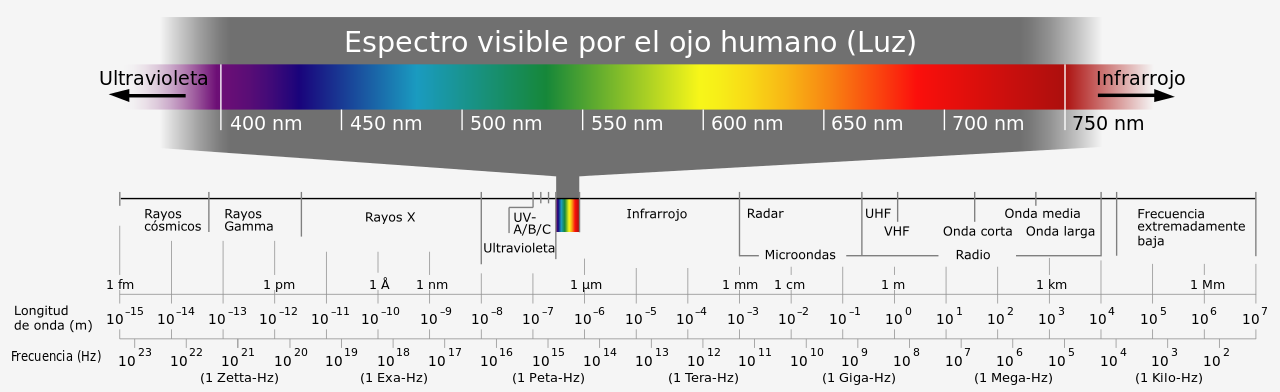
\includegraphics[scale=.3]{images/espectro}
  \caption{\em Luz visible por el ojo humano en el espectro electromagnético~\citep{Horst2006}. }  
  \label{fig:espectro}
\end{figure}

Cuando la luz incide sobre un objeto, puede ser absorbida y la energía, convertida en calor, puede atravesarlo o bien ser reflejada por el mismo. El color de un objeto depende de la cantidad relativa de luz absorbida y de luz reflejada, los objetos de colores reflejan luz que tiene una mayor densidad ondas para ciertas de longitudes de onda del espectro visible que en otras. 

\begin{figure}[h]
  \centering
  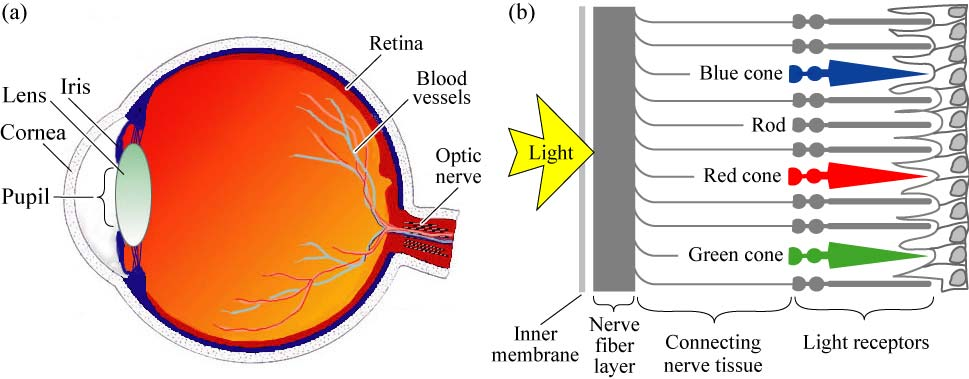
\includegraphics[scale=.4]{images/ojo}
  \caption{\em A la izquierda anatomía del ojo humano, a la derecha esquema de la retina, que muestra conos y bastones. Adaptado de \cite{Britannica1994}}  
  \label{fig:ojo}
\end{figure}

La luz debe atravesar el ojo (figura~\ref{fig:ojo}), desde la córnea hasta la retina, generando un enfoque con la menor distorsión posible. La retina consta de diez capas que trabajan en conjunto con la finalidad de generar el impulso nervioso que se dirigirá a la corteza cerebral para reconocer finalmente una imagen. El ojo es capaz de absorber la luz en su totalidad e impedir la reflexión en su interior, siendo ésta transmitida hacia la segunda capa de la retina, conformada por los foto-receptores, células sensoriales sensibles a la intensidad y longitud de onda de la luz. Existen dos tipos; conos y bastones. Los bastones, elementos encargados de la visión con poca luz, son acromáticos, es decir, sólo permiten captar la luz en tonalidades de gris. Tienen un pico de sensibilidad aproximado en los 500 nm, como se puede observar en la figura~\ref{fig:cono} (curva R). Los conos por su parte, son los elementos encargados de activarse en condiciones de alta intensidad lumínica, por lo que generan la visión cromática diurna. Hay tres clases de conos, distintos entre sí por el tipo de pigmento fotosensible que contienen. Los pigmentos en los tres tipos de conos contienen picos de absorción de luz según la longitud de onda. Éstos se encuentran aproximadamente en 420 nm (receptores para el violeta – azul, conos S), 530 nm (receptores para el azul – verde, conos M) y 560 nm (receptores para el amarillo – verde, conos L). Los tres grupos de conos mezclados generan el espectro completo de luz visible. En capas posteriores se codifica la información recibida, la cual es enviada a través de dos nervios ópticos por cada ojo en dirección hacia el cerebro.

\begin{figure}[h]
  \centering
  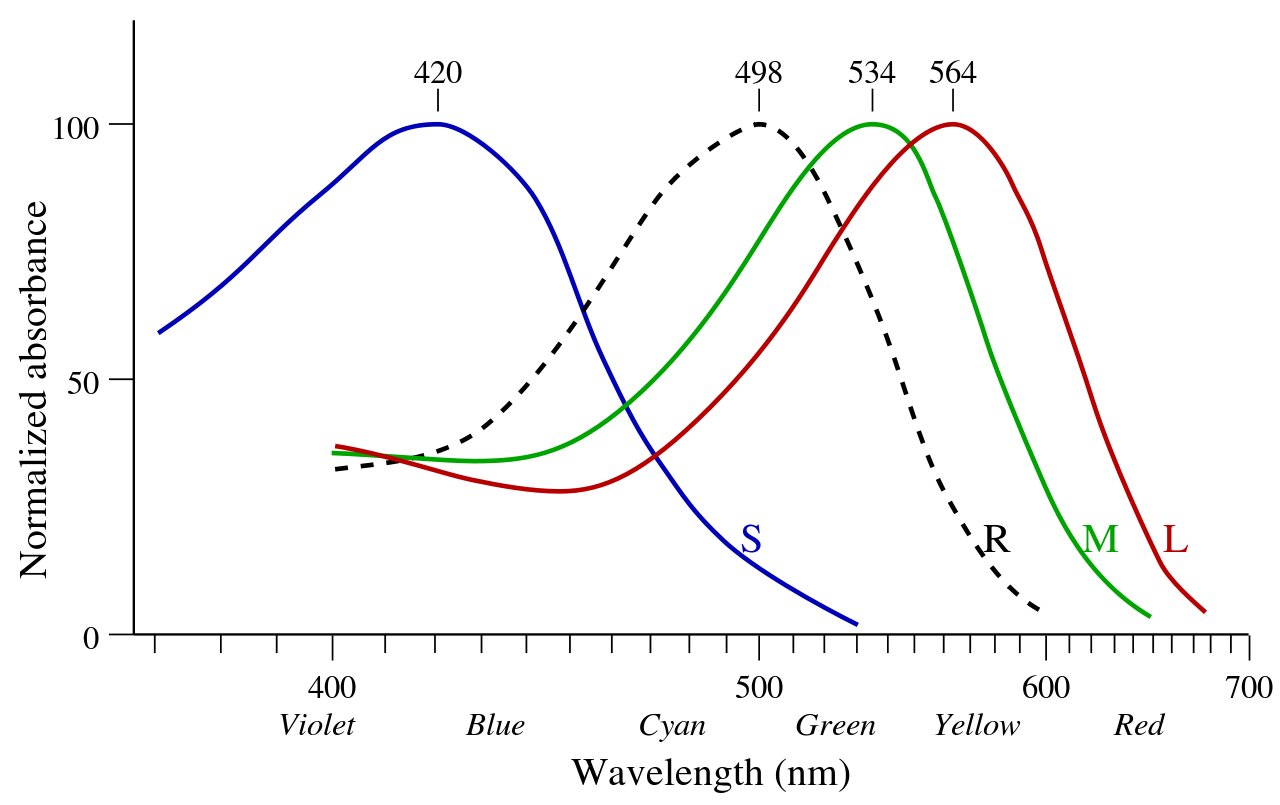
\includegraphics[scale=.3]{images/cono}
  \caption{\em Curvas de absorción espectral de corta (S), mediana (M) y larga (L) longitud de onda,según pigmentos de células cono y bastones (R) humano. Adaptado de \cite{Bowmaker1980}}  
  \label{fig:cono}
\end{figure}

En su trayectoria, los dos nervios ópticos centrales se entrecruzan, para generar procesamiento de información de ambos ojos en cada hemisferio cerebral, tal como puede observarse en los trayectos en verde en la figura~\ref{fig:cerebro}. Este proceso es importante para la visión de profundidad. Posteriormente se dirige a través del tracto óptico, información proveniente de ambos ojos hacia la corteza visual primaria, ubicada en el lóbulo occipital. Desde allí, se comunican con la corteza visual de asociación, responsables del reconocimiento de objetos y de la percepción del color.

\begin{figure}[h]
  \centering
  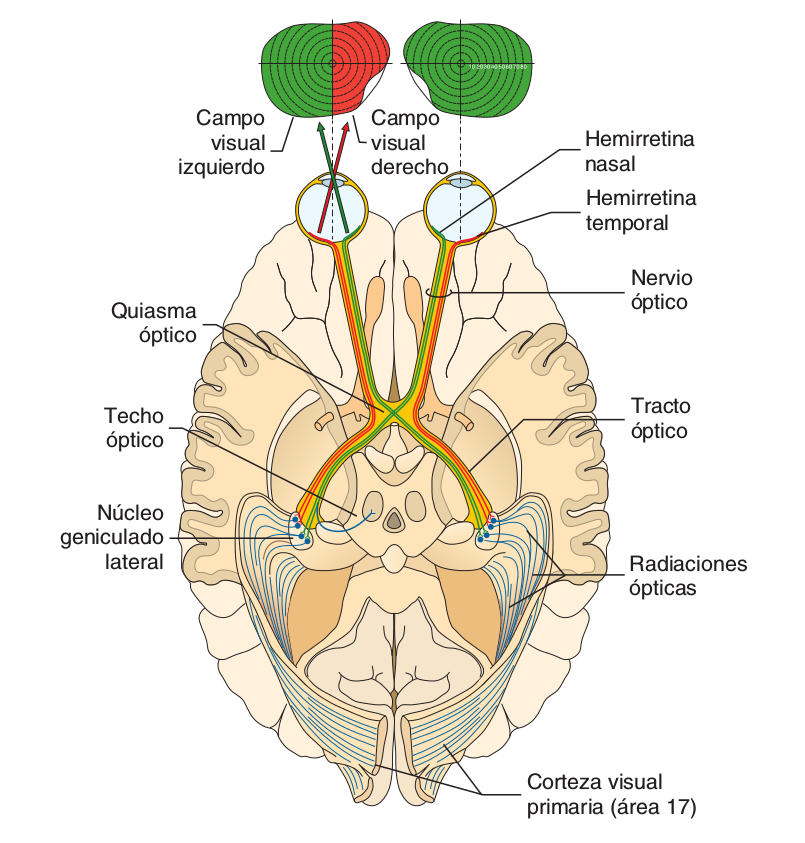
\includegraphics[scale=.3]{images/cerebro}
  \caption{\em Principales vías visuales. Obtenido de \cite{Battaglini2010}}  
  \label{fig:cerebro}
\end{figure}

Este proceso toma en un ser humano desde fracciones hasta unos cuantos segundos, sin embargo, utilizar un computador para realizar dicho ejercicio se torna una tarea desafiante. La visión por computador es un área de estudio que trata este problema. Corresponde a un campo dentro de la inteligencia artificial enfocado al modelamiento matemático de los procesos de percepción visual de los humanos. En general está enfocada al procesamiento de las imágenes con el fin de obtener información simbólica de estas. Algunas de las tareas que pretende resolver la visión por computador son determinar la posición, la distancia o contar los objetos en una imagen. En palabras sencillas la visión por computador se enfoca en la tarea de ``enseñar a ver a los computadores''.

\begin{figure}[h]
  \centering
  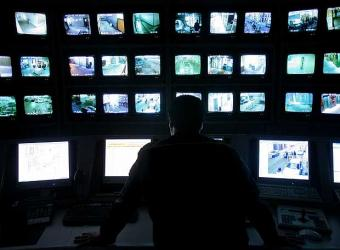
\includegraphics[scale=.42]{images/vigilancia}
  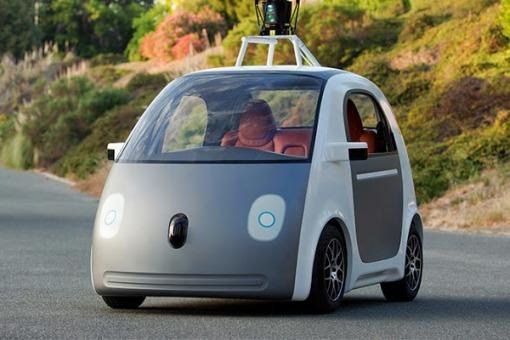
\includegraphics[scale=.36]{images/googleauto}
  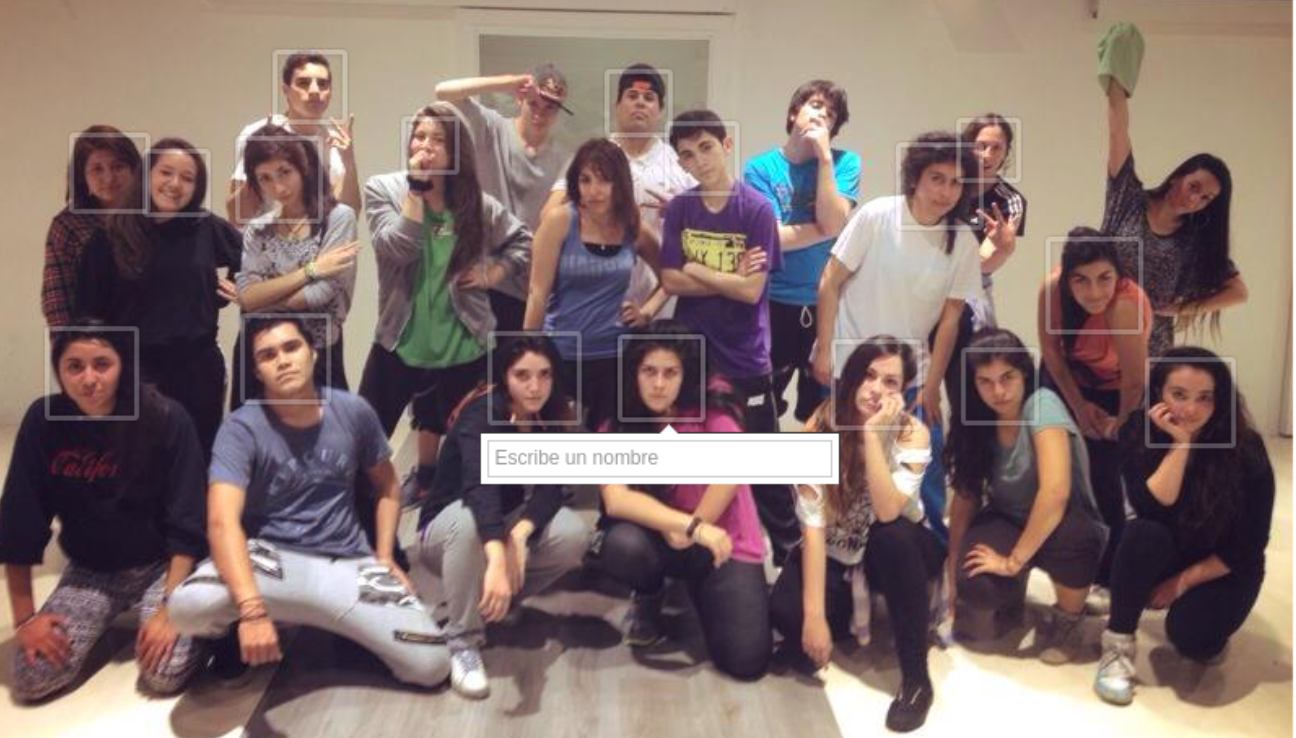
\includegraphics[scale=.25]{images/faces}
  \caption{\em Algunos ejemplos de aplicaciones de la visión por computador. Arriba a la izquierda sistema de video vigilancia. Arriba a la derecha auto autónomo inteligente de Google. Abajo reconocedor de rostros de Facebook}  
  \label{fig:ejemplosaplicacion}
\end{figure}

Existe una gran variedad de investigaciones en el área de la visión por computador, pero sin duda uno de las principales tareas corresponde a la detección de diferentes tipos de objetos en imágenes y videos. El desarrollo de esta capacidad en un computador abre las puertas a un gran número de aplicaciones en variadas áreas como; interacción humano-computador, robótica, análisis automático de contenido en medio digitales, automatización de proceso de manufactura y automóviles autónomos inteligentes.

El presente trabajo centra su foco en un problema particular dentro de la detección de objetos, el cual es, la detección de personas. Y más aún un subproblema dentro de la detección de personas, la caracterización de la ``Sensibilidad Espacial''. Para solucionar el problema de la detección de personas se ha propuesto diversidad de enfoques. Algunos de los enfoques más relevantes del problema son la detección holística \citep{dalal2006}  que corresponde a la consideración de la persona de cuerpo completo como un todo, la detección basada en partes \citep{nevatia2005} detectando partes de un objeto por separado y luego reuniéndolas, o una mezcla de estos enfoques \citep{leibe2005,yu2011}.

El problema de determinar la existencia de un peatón en una determinada ventana de clasificación se encuentra bien estudiado. Sin embargo, al considerar un enfoque de detección basado en un ventana deslizante que se desplaza por la imagen realizando clasificaciones para encontrar a un peatón, surge la posibilidad de que se realicen múltiples detecciones. Esta probabilidad aumenta cuanto más cerca este la ventana respecto del objeto a detectar. Como es preciso evitar que esto ocurra es necesario estudiar el comportamiento de la salida del clasificador, especialmente en la cercanía del peatón. A las variaciones en la salida mientras se desplaza la ventana de clasificación se le denomina ``Sensibilidad Espacial''.

Como se explica con detalle más adelante, la Sensibilidad Espacial es un concepto clave dentro del desarrollo de este trabajo ya que es importante su caracterización (para una determinada combinación de descriptor y máquina de aprendizaje) de modo que sea posible determinar cual es el grado de sintonización del clasificador respecto de los objetos que se encuentra clasificando.

\section{Descripci\'on del problema}
\label{intro:problema}

Determinar la existencia de un peatón en una sección de una imagen es un problema bastante estudiado. Sin embargo, dentro de la detección de peatones (donde están los peatones en una imagen) se encuentra el subproblema del comportamiento del clasificador en el momento de encontrarse evaluando la vecindad cercana al peatón. A este problema lo denominamos caracterización de la sensibilidad espacial.

Un clasificador de personas (o cualquier otro tipo de objeto para los cuales haya sido entrenado) evalúa la presencia de un peatón en la imagen analizando la información tomada de una ventana o cuadro que se desliza por dicha imagen y entrega como resultado la determinación de la existencia de un peatón o no además de un valor para el nivel de confianza con el cual el clasificador asegura que se trata de un peatón.

\begin{figure}[H]
  \centering
  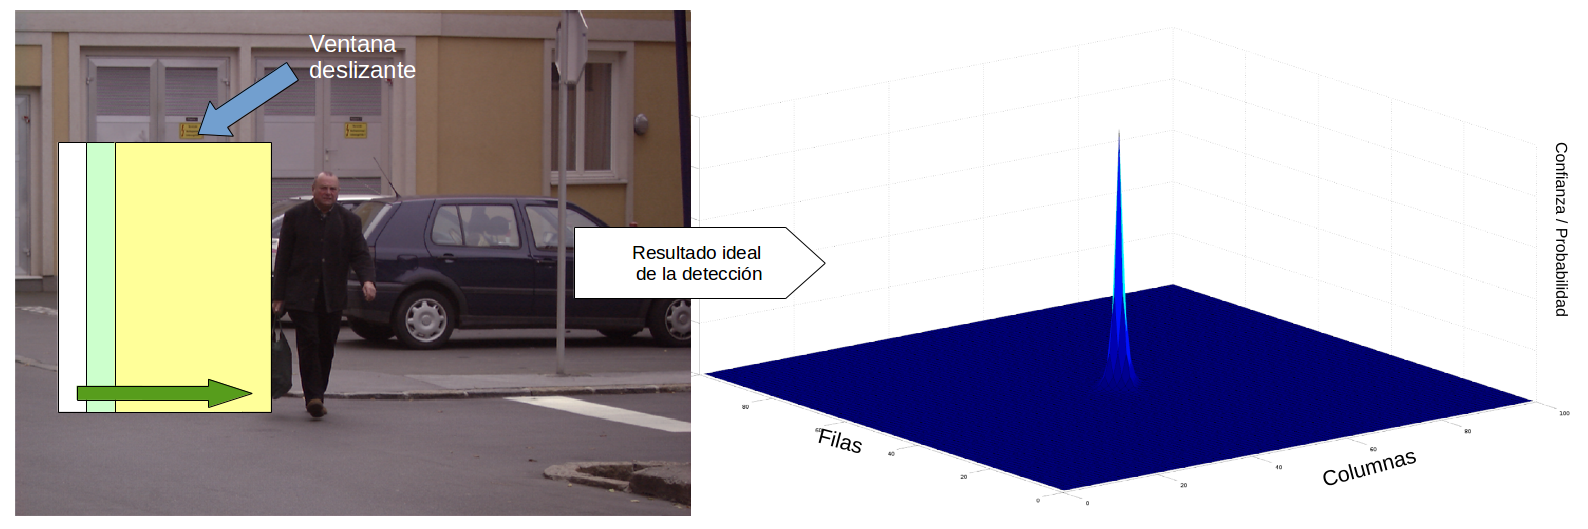
\includegraphics[scale=.3]{images/ejloesp}
  \caption{\em Escenario ideal en la salida de un clasificador. A la izquierda detección con la ventana deslizante. A la derecha salida ideal.} 
  \label{fig:ejloesp}
\end{figure}


En forma ideal, la confianza de la respuesta del clasificador sólo debe ser muy alta cuando la ventana evaluada se encuentra frente a frente al peatón y no cuando se encuentra en su cercanía. En este último caso, la confianza de su respuesta debe ser muy baja. En la figura~\ref{fig:ejloesp}, a la izquierda se observa en color verde el desplazamiento de la ventana de clasificación acercándose al momento en que la ventana se encuentre completamente frente al peatón, a la derecha se muestra el resultado obtenido posterior a la clasificación desplazando la ventana por toda la vecindad. Si se tratase de un buen clasificador; en un escenario ideal el resultado obtenido debería asemejar a la función impulso. Esta es entonces una posible representación de un escenario ideal.


\section{Soluci\'on propuesta}
\label{intro:solucion}
% ***SAV here 

\subsection{Características de la solución propuesta}

Para caracterizar la sensibilidad espacial se propone por una parte una métrica y por otra una metodología de evaluación. Tanto la métrica como la metodología de evaluación se construirá de modo que pueda ser implementada basada en la biblioteca de visión por computador OpenCV. Esta biblioteca contiene implementaciones de varios algoritmos de visión por computador además de herramientas para el manejo de imágenes en general. También existen desventajas en la utilización de OpenCV ya que la documentación asociada a la biblioteca se encuentra incompleta y presenta una cantidad apreciable de errores, lo que dificulta su utilización.

La evaluación será desarrollada en torno a una métrica propuesta, lo que se construirá en una serie de siete pasos con la culminación del cálculo de la propia métrica. Es importante que durante la evaluación sea posible obtener resultados parciales para comprobar el avance y contrastar diferencias. El enfoque principal de la evaluación será realizar una detección del peatón en base al modelo de la ventana deslizante en su vecindad. 

Por el lado de la métrica es importante que cumpla con la mayor cantidad de características deseables de una métrica. Algunas de estas características son.

% ***SAV. A lo mejor debes tener un poco de cuidado con la palabra "metrica" ya que matematicamente es bastante más precisa de lo que usas (ver http://es.wikipedia.org/wiki/Espacio_m%C3%A9trico) . A lo mejor debes aclarar que lo que buscas es una "medida" más que una metrica estricta o mejor aun si demuestras que tu metrica es de verdad una metrica (no debiera ser muy complicado) ***DQ Revisado

\begin{itemize}
\item Fácil de medir: toda métrica debes aspirar a ser fácil de medir, cuanto más fácil más extendido será su uso y más rápido será perfeccionada.
\item Linealidad: idealmente la métrica debe ser lineal respecto de la característica a medir.
\item Fiabilidad: la métrica debe aumentar o disminuir su valor conforme aumenta o disminuye la propiedad medida respectivamente. También esta variación puede ser inversa \ie mientras una aumenta la otra disminuye.
\item Repetibilidad: al realizar el mismo experimento en varias ocasiones el resultado es el mismo \ie la métrica tiene un resultado determinista.
\item Consistencia: al cambiar el sistema y la configuración la métrica debe mantener su significado y su unidad de medida.
\item Independencia: la métrica no debe estar influenciada para obtener resultados de algún tipo en especifico.
\end{itemize}

Además, matemáticamente una métrica es una función distancia asociada a un espacio métrico que debe cumplir cuatro axiomas, estos son: positividad, identidad de los indiscernibles, simetría, desigualdad triangular. Entonces es necesario demostrar que la métrica diseñada cumpla con estos axiomas. 

\subsection{Propósitos de la solución}

El propósito de la solución es contribuir a la investigación en detección de peatones. Para esto se caracterizan nuevos aspectos del problema antes no tratados. La detección de peatones es un problema muy amplio por lo que una contribución tiene repercusión a nivel de una gran gama de aplicaciones distintas. 
De forma directa esta investigación realiza un aporte dentro del proyecto Fondecyt Regular OBSERVE (N'o 1140209), orientado al reconocimiento de acciones humanas dentro del transporte público.

Otro propósito lateral es aportar en problemas similares de detección no necesariamente relacionada con personas \ie detección de objetos en general. Muchos algoritmos de detección de objetos están basados en la misma estructura que un detector de personas por lo que es perfectamente aplicable esta solución en esos problemas.

\section{Objetivos y alcance del proyecto}
\label{intro:objetivos}

\subsection{Objetivo general}

Desarrollar una metodología que permita la comparación y un software de pruebas que permita la evaluación sistemática de múltiples clasificadores con el fin de encontrar aquel con mejor sensibilidad espacial, para minimizar detecciones múltiples en la vecindad del peatón utilizando el set de datos INRIA

%**DQ Desarrollar y probar una métrica que permita la comparación de la sensibilidad espacial entre diferentes esquemas descriptor-clasificador, encontrando aquel que reduce detecciones múltiples en la vecindad del peatón utilizando el set de datos INRIA.

\subsection{Objetivos específicos}

Para la consecución del objetivo general, se plantean las siguientes metas intermedias:

\begin{enumerate}
\item Crear un modelo matemático que permita generar un indicador que describa la sensibilidad espacial según la respuesta de los clasificadores.
\item Diseñar una metodología de evaluación de la sensibilidad espacial de un clasificador en la vecindad de un peatón.
\item Desarrollar un software modular que permita la automatización de la metodología y la comparación de clasificadores.
\item Implementar los descriptores y clasificadores que no se encuentren previamente implementados para su evaluación.
\item Determinar cuál de los clasificadores corresponde al que posee la mejor sensibilidad espacial para minimizar detecciones múltiples de peatones en el set de datos INRIA.

%**DQ \item Proponer un modelo matemático que permita generar un métrica que describa la sensibilidad espacial.
%\item Realizar de evaluación de la sensibilidad espacial de un clasificador en la vecindad de un peatón.
%\item Desarrollar un software modular que permita la automatizar la evaluación de la sensibilidad espacial para cada peatón del ``ground truth''. 
%\item Implementar los descriptores y clasificadores que no se encuentren previamente implementados para su evaluación.
%\item Determinar cuál de los clasificadores corresponde al que posee la mejor sensibilidad espacial para minimizar detecciones múltiples de peatones en el set de datos INRIA.

\end{enumerate}

\subsection{Alcances y limitaciones}

Los alcances y limitaciones listados a continuación ayudan a determinar la frontera del proyecto. 

\subsubsection{Alcances}

Para efectos de la evaluación de los clasificadores humanos se utilizó un set de datos único, que corresponde al set de datos INRIA. Este estudio comprende la caracterización de la sensibilidad desde un enfoque métrico \ie el objetivo es medir la sensibilidad espacial. Esta incluido en el desarrollo una etapa de para la proposición de la métrica, una para la evaluación diseño del proceso de evaluación, una etapa para el desarrollo de software y finalmente una etapa para realizar el análisis comparativo y la escritura del presente documento.

\subsubsection{Limitaciones}

\begin{itemize}

\item Está fuera de los alcances del proyecto el desarrollo de nuevas técnicas o algoritmos de clasificación, se busca probar los algoritmos existentes en su estado original o modificar sus variables de manera que mejore su sensibilidad espacial según el indicador obtenido.

\item La solución de software corresponde a un programa para línea de comandos desarrollado para sistema operativo Linux y no se considera dentro de la solución el desarrollo de ningún tipo de interfaz gráfica adicional.

\item Se realizó el análisis de 8 combinaciones de descriptor-clasificador en diferentes escalas dentro de las cuales algunas se encuentran implementadas y otras deberán ser implementadas previo a realizar las pruebas.

\item Finalmente la solución se validó ya que el software construido tiene la capacidad de probar diferentes clasificadores humanos entregando sus resultados, el valor del indicador comparativo y es posible determinar la sensibilidad espacial de cada uno permitiendo su comparación.

\end{itemize}

%**DQ REVISAR METODOLOGÍA!!

\section{Metodolog\'ia y herramientas utilizadas}
\label{intro:metodologia}

Para el desarrollo del trabajo en se realiza fundamentalmente un proceso de investigación el cual lleva incorporado dentro de si una etapa de desarrollo de software por esta razón es importante conocer el marco metodológico asociado a la investigación y en forma secundaria aquel relacionado con el desarrollo de software.
El proceso de investigación tiene gira en torno a la posibilidad de evaluar la sensibilidad espacial dada una clasificación en torno a la vecindad de un peatón y comparar este resultado con el resultado obtenido por un clasificador diferente.

\subsection{Metodología para la investigación}

La metodología de investigación funciona como marco general para el desarrollo por lo que es necesario cumplir un objetivo científico \ie describir y evaluar la sensibilidad espacial a través de una métrica propuesta. Para esto se utilizará el método científico.

Las actividades dentro de esta metodología son las que se describen a continuación.

\begin{itemize}
\item Formulación de la hipótesis. 
La hipótesis formulada tiene relación directa con el correcto funcionamiento de la métrica la que debe permitir diferenciar resultados de un conjunto descriptor-clasificador de los de otro. Para esto es necesario plantear una hipótesis como la siguiente.
\subitem ``La métrica propuesta permite la comparación de los resultados de sensibilidad espacial entregando resultados con diferencias estadísticamente significativas''
\item Marco teórico. Explicar conceptos básicos sobre visión por computador y cuales son las principales áreas de estudio relacionadas. Exponer la investigación sobre detección de peatones así como las herramientas, métodos y enfoques asociados.
\item Diseño de la solución. Realizar la proposición de un una métrica que permita evaluar la sensibilidad espacial y diseñar el proceso de evaluación con el cual se validará. Además se describirán las herramientas seleccionadas para la evaluación de la métrica y se fundamentará las razones de su elección.
\item Análisis y presentación de los resultados. Se realizará el análisis de los resultados obtenido mostrando el proceso de comparación a nivel gráfico y por otra parte el análisis estadístico el cual permite finalmente la aceptación o rechazo de la hipótesis planteda.   
\item Conclusiones. Se presentan las conclusiones sobre los resultados obtenidos.

\end{itemize}

\subsection{Metodolog\'ia para el desarrollo de software}

%%POR COMPLEMENTAR !!!!!

Dada la necesidad de construir una solución de software que permita incorporar tanto el proceso de detección de peatones como el  evaluación de la sensibilidad espacial. Sin embargo esta metodología debe adaptarse a las necesidades cambiantes de la investigación y tener por objetivo principal obtener rápidamente los resultados necesarios para probar adecuadamente la hipótesis planteada.

En primer lugar, dada la naturaleza de este trabajo, el equipo de desarrollo se compuso de un solo integrante – el autor – quien además funcionó como cliente conjunto con la colaboración del profesor guía. Entonces es él quien identifica los requerimientos asociados a la solución de software a desarrollar y quien debe darle posterior cumplimiento. En segundo lugar se considera que las necesidades de documentación del software eran necesarias en lo que respecta a usuarios y desarrolladores externos que desearan observar su trabajo, pero que el número de artefactos a utilizar no debía ser extenso, principalmente por la poca practicidad que representa el uso de muchos de ellos. Se prefirió entonces la utilización de una metodología ágil que permitiera optimizar la utilización del recurso tiempo y que fuera adaptable a cada que pudiera presentarse situación. Es por esta razón que se escogió como metodología de desarrollo a \textit{Extreme Programming} (XP) adaptado a una sola persona.

Se justifica la elección de XP debido principalmente al hecho de que constituye una metodología ágil que permite centrar el foco principalmente en el desarrollo de la solución más que en la construcción de artefactos, se puede adaptar de manera sencilla a un equipo unipersonal donde se cumple con la particularidad además de que el cliente y el equipo de desarrollo son la misma persona, asegurando de esta forma un 100\% de disponibilidad y comunicación entre ambos roles de la metodología (que asume que el cliente está siempre presente durante el desarrollo del proyecto).

Si bien el proyecto no se consideró como de alto riesgo, la metodología, gracias a los ciclos de desarrollo cortos y pruebas constantes, permite minimizar el riesgo asociado al desarrollo detectando y controlando los fallos en el desarrollo, tanto a nivel de código como de planificación de manera temprana y con consecuencias reducidas, presentando una considerable ventaja por sobre otras metodologías bajo las circunstancias en las cuales se llevó a cabo el desarrollo.

\subsection{Herramientas de desarrollo}

Para el desarrollo de este proyecto de título fue necesaria la utilización de herramientas que permitieron llevar llevar a cabo tanto la construcción del software relacionado como la redacción del presente documento.
En particular para el desarrollo del software se utilizaron las siguientes herramientas.

\begin{itemize}
  \item SublimeText 3 - Procesador de texto con variadas utilidades para la producción de código.
  \item C++ 11 - Lenguaje de programación C++ en su estándar del año 2011 ISO/IEC 14882:2011.
  \item OpenCv 2.4 - Biblioteca open source para el desarrollo de aplicaciones de visión por computador, con soporte para c, c++ y python.
  \item Boost C++ Libraries 1.5 - Biblioteca para C++ con importantes mejoras para el lenguaje.
  \item Python - Lenguaje de programación python en su versión 2.7.6.
  \item Octave - Lenguaje de programación interpretado de alto nivel, similar a MATLAB, en su versión 3.8.1.
  \item Linux Mint 17 - Sistema operativo linux basado en Ubuntu 14.04.
  \item Git - Herramienta para el control de versión de código, se utilizó el servicio prestado por Github para mantener una copia en linea.
  \item OpenMP - API para programación paralela para lenguaje de programación C/C++.
  \item SPSS 22.0 - Software para análisis estadístico predictivo de IBM 
  \item STATISTICA 10.0 - Software para análisis estadístico predictivo de StatSoft - Dell Software
\end{itemize}

Para la escritura del presente documento se utilizaron las siguientes herramientas

\begin{itemize}
\item Latex - Para el procesamiento, compilación del texto y transformación en pdf.
\item Dropbox - Para almacenamiento en línea y control de versión.
\item Sharelatex - El servicio de sharelatex provee un entorno de escritura además de las facilidades para la compilación y sincronización con dropbox.
\end{itemize}


\section{Organizaci\'on del documento}
\label{intro:organizacion}

El presente trabajo está dividido en siete capítulos considerando éste como el primero. En el capítulo~\ref{cap:preliminares} se ilustrará el marco teórico y el estado del arte en torno al problema antes descrito, a continuación en el capítulo~\ref{cap:metricas} se analizará el proceso por el cual fueron seleccionadas las métricas de sensibilidad espacial y como se construye cada una de estas. A continuación en el capítulo~\ref{cap:caract} se evaluarán las técnicas utilizadas para la extracción de características de las imágenes en particular del algoritmo HOG. En el capítulo \ref{cap:eval} se expone el proceso de evaluación realizado a través del  cual se obtuvieron los resultados que son expuestos en el capítulo \ref{cap:analisis}. Además en el capítulo \ref{cap:analisis} se realiza el análisis comparativo de los clasificadores analizados. Finalmente en el capítulo \label{cap:conclusiones} se realiza una breve discusión, se concluye sobre los resultados obtenidos y la proyección de es estos para futuras investigaciones.

Para mejorar la lectura del presente documento se puede encontrar cuatro anexos los cuales contienen, el manual de usuario del software desarrollado, los gráficos obtenidos al realizar análisis de métricas, los gráficos obtenidos para el análisis comparativo y finalmente un glosario con explicaicones de los conceptos mas importantes.

%--------Preliminares
%--------Daniel Quinteros Céspedes
%--------23-09-2014

\chapter{Marco Te\'orico}
\label{cap:preliminares}

En el capítulo anterior se revisó el contexto general del problema, en el presente capítulo se dará paso a la explicación de los conceptos teóricos más relevantes que se relacionan con el trabajo expuesto en el presente documento. Algunos de ellos son la visión por computador, los elementos del procesos de detección de peatones y la sensibilidad espacial.

\section{Visión por computador}
\label{preliminares:cv}

Existen variadas definiciones sobre lo que se trata la visión por computador, \cite{mery2004} indica en su libro ``Visión por Computador'' algunas de las definiciones más relevantes enunciadas por expertos en el área.

\begin{itemize}
\item ``Ciencia que desarrolla las bases teóricas y algorítmicas para obtener información sobre el mundo real a partir de una o varias imágenes''~\citep{haralick1992}.
\item ``Disciplina que desarrolla sistemas capaces de interpretar el contenido de escenas naturales''~\citep{kennethr.1996}.
\item ``La Visión por Computador, que ha emergido como una disciplina propia basada principalmente en las matemáticas y ciencias de la computación consiste en hacer que un computador vea. Esto sin embargo es todavía un problema no resuelto\ldots''~\citep{hartley2003}.
\end{itemize}

La visión por computador o en inglés \textit{computer vision}, es entonces un campo de estudio dentro del área de la inteligencia computacional el cual se dedica al análisis y comprensión de la imágenes en general. El objetivo principal es emular la forma en la que el ojo humano (o el de otro ser vivo) es capaz de extraer e interpretar información de las imágenes, para esta tarea se vale del modelamiento matemático, la computación y la electrónica como principales herramientas. 

\begin{figure}[tp]
  \centering
  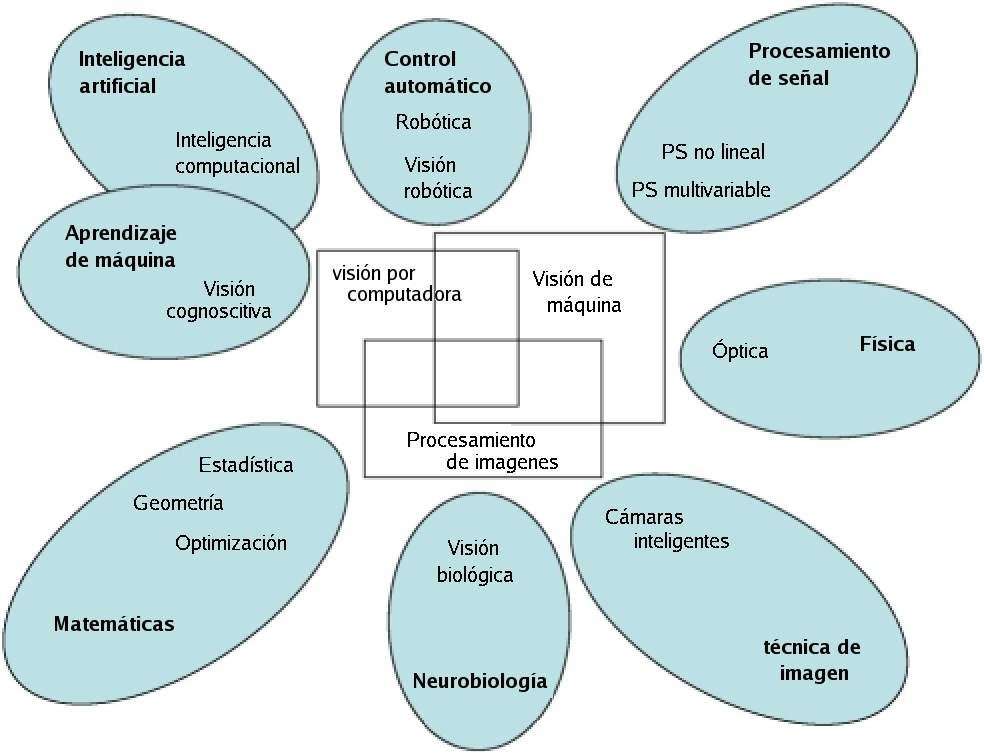
\includegraphics[scale=.3]{images/cv-context}
  \caption{\em Visión por computador y áreas afines.}  
  \label{fig:cvcontext}
\end{figure}

La visión por computador se encuentra rodeada de una gran cantidad de áreas de investigación de las cuales se ve nutrida (figura~\ref{fig:cvcontext}). Esta variedad de áreas afines implican una gran cantidad de potenciales aplicaciones relacionadas. Sin embargo, en general el proceso de procesamiento por el que pasan las imágenes es posible generalizarlo. Como se muestra en la figura~\ref{fig:cvprocess} el proceso se inicia con la adquisición de la imágenes obteniendo una imagen del objeto que se desea estudiar, luego en el pre-procesamiento se hace uso de algunos filtros digitales que permiten eliminar el ruido o eliminar el contraste con el objetivo de mejorar la calidad de esta, luego en la etapa de segmentación se realiza la identificación del objeto de estudio del resto de la imagen, en la medición o extracción de características se realiza una medición de los atributos de interés de la imagen y finalmente en la interpretación, se clasifica o etiqueta al objeto, es importante señalar el foco del presente documento se encuentra en esta última etapa y busca mejorar una parte del proceso de interpretación.

\begin{figure}[tp]
  \centering
  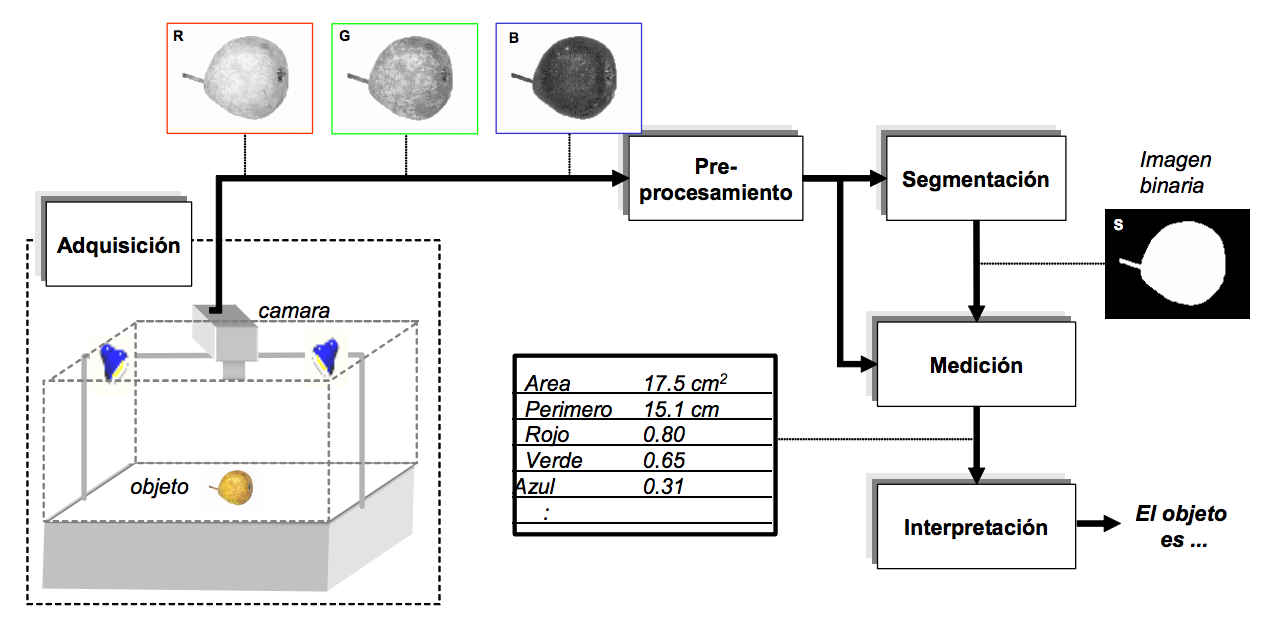
\includegraphics[scale=.3]{images/cv-system}
  \caption{\em Esquema de un proceso de análisis de imágenes.} 
  \label{fig:cvprocess}
\end{figure}

\section{Set de datos de peatones INRIA}
\label{preliminares:deteccion}

El set de datos de personas de INRIA, construido por \cite{dalal2005}, corresponde a una colección de imágenes de peatones en distintos formatos utilizado para el entrenamiento y pruebas del sistema solución. Está compuesto principalmente de imágenes provenientes de tres fuentes: el dataset de la Universidad Tecnológica de Graz, colecciones de imágenes personales del autor y Google Web Images. En todas estas imágenes aparecen personas de pie, y no todas las anotaciones son correctas, esto significa que para algunos casos, el recuadro de delimitación (\textit{bounding box}) puede estar desplazado respecto del objeto. En total el set de datos  contiene 
Las imágenes se presentan en dos formatos: las imágenes originales con sus archivos de anotaciones asociados, y las imágenes en positivo normalizadas a formato de 64x128 píxeles con las imágenes en negativo originales asociadas. Las imágenes originales están organizadas en una carpeta de entrenamiento y una carpeta de pruebas, y dentro de cada una de ellas, las carpetas pos, que contiene las imágenes en positivo, neg, que contiene las imágenes en negativo, y annotations, que contiene las anotaciones para las imágenes. Por su parte, las imágenes normalizadas se dividen en dos carpetas, pos y neg, las que siguen la misma lógica de nombres que las imágenes originales.
Utilizando este conjunto de datos, el sistema solución puede ser entrenado para así poder llevar a cabo la tarea de detección de personas. En el siguiente paso se revisará información sobre los algoritmos utilizados para extraer información de las imágenes

\section{Características de las imágenes}
\label{preliminares:caract}

Para cualquier tarea de detección es necesario obtener información de la imagen que permita diferenciar un objeto de otro o una persona de otra, en este punto entran las técnicas de extracción de características que entregan como resultado simbología que permite a un computador interpretar lo que esta ``viendo''. En un escenario ideal estas características deberían representar a un objeto en la imagen y permanecer constante durante cambios de iluminación, cambios de punto de vista o cambios en el borde de los objetos. Para lograr esto se han desarrollado distintos enfoques, \cite{dalal2006} indica que estos enfoques se pueden agrupar en dos categorías o enfoques diferentes. La primera categoría, representaciones dispersas incluye detección basada en puntos, en fragmentos de la imagen y en partes. La segunda categoría es la de representaciones densas y utiliza la intensidad de la imágenes o gradientes.

\subsection{Representaciones locales dispersas}
\label{caract:dispersas}

Las representaciones dispersas intentan describir las características de la imagen utilizando regiones localizadas de la imagen. Comúnmente estas regiones son seleccionadas utilizando uno de dos enfoques: detección de puntos clave o detección de partes. A continuación se revisará brevemente ambos enfoques.

\subsubsection{Detectores de puntos clave (\textit{keypoints})}

La idea esencial detrás de los detectores basados en puntos clave (\textit{keypoints}) es que son capaces de seleccionar regiones estables y fiables de la imagen las cuales contienen información muy representativa del contenido local de la imagen. Entonces, los detectores cuyo enfoque esta basados en puntos clave tienen por objetivo extraer de la imagen un pequeño conjunto de puntos sobresalientes de la imágenes o puntos de interés, estos puntos de interés son procesados para obtener vectores de características de ellos los que a su vez permiten, finalmente, la construcción del detector. Las principales ventajas del uso de detectores basado en puntos clave es su tamaño, el cual es considerablemente más pequeño que la cantidad de píxeles en la imagen lo que permitiría un procesamiento más rápido en las últimas etapas del proceso de detección. En general el desempeño de los detectores basados en puntos clave depende de que tan informativos sean los puntos encontrados y si para una clase determinada es posible encontrar estos puntos de una forma fiable, precisa y repetible. Algunos de los enfoques más populares \citep{gupta2008} en cuanto a los puntos clave son \textit{Scale Invariant Feature Transformation} (SIFT) \citep{Lowe2004}, el cual resuelve unos de los problemas más relevantes de la detección por puntos clave: la invariabilidad frente al escalado; \textit{Gradient Location and Orientation Histogram}~(GLOH)~\citep{Mikolajczyk2005}, este descriptor es una mejora de SIFT que busca mejorar la robustez y el grado de diferenciación; \textit{Shape context}~\citep{Belongie2002}, es una manera de describir la forma que permite medir la similitud y recuperar la correspondencia de los puntos; \textit{Speeded Up Robust Features} (SURF) \citep{Bay2006}, es esencialmente un algoritmo inspirado en SIFT y pensado para mejorar el tiempo de computo; PCA-SIFT~\citep{Ke2004}, es también una mejora de SIFT que esta vez utiliza análisis de componentes principales (PCA) haciendo más compacto al descriptor.

% ***SAV: no entiendo el párrafo siguiente !!!
Aún cuando la utilización de detectores basados en puntos clave se encuentra ampliamente extendida dentro del problema de detección de objetos, presenta un problema característico. Este tipo de detectores se encuentran diseñados para encontrar repetidamente un mismo objeto en una imagen por lo surgen problemas cuando el objeto se generaliza en clases o categorías.


\subsubsection{Detectores basados en partes o extremidades}

La detección basada en partes así como la basada en puntos clave también tiene un uso extendido en los sistemas de detección de peatones. Para este caso en particular de detección existen también distintos enfoque. Sin embargo, la ideea principal detrás de la detección basada en partes es que las partes o extremidades pueden ser representadas de forma geométrica. Existen enfoques en los cuales se asume que cada parte de cuerpo como, antebrazo, brazo, torso, etc.  puede representarse bien utilizando un cilindros \citep{Ramanan2003}. Otros tipos de construcciones geométricas también han sido utilizadas para este fin, por ejemplo usando detección de bordes para obtener modelos relativos de la extremidades. Otros enfoques utilizando este tipos de descriptores son los detectores de extremidades 3D \citep{Sigal2003}. En general estos descriptores funcionan bien, sin embargo presentan algunos problemas, pues la simplicidad de la representaciones geométricas con lineas son difíciles de extrapolar a la complejidad del mundo real.


\subsection{Representaciones densas de las regiones de una imagen}
\label{caract:densas}

Las representaciones locales tienen en general una ventaja respecto de la velocidad de cómputo. Sin embargo, al ser locales pueden perder la perspectiva, por lo que es importante revisar su contrapartida, en este caso, las representaciones densas. En general estas representaciones obtienen una cantidad de características muy grande incluso tantas como píxeles haya para una imagen entera o un ventana de detección obteniendo vectores descriptores con una alta dimensionalidad el cual puede ser utilizado para realizar un clasificación. 
A continuación se explicarán algunos enfoques relacionados con este tipo de representaciones, que están generalmente basadas en la utilización de intensidades de la imagen, gradientes u operadores diferenciales.

\subsubsection{Regiones basadas en la intensidad de la imagen}

Aún cuando en general los detectores basados en la intensidad de la imagen han sido utilizados principalmente para la obtención de puntos clave en representaciones locales dispersas, también existen algunos ejemplos en representaciones densas. Según \cite{dalal2006}, una de los primeras propuestas de este tipo de descriptores corresponden a las realizadas por \cite{Sirovich1987} y \cite{Turk1991} utilizando intensidades simples de la imagen. Este enfoque se conoce como \textit{``eigenfaces''} y el mismo autor señala también la existencia de otros dos enfoques. El primero para el desarrollo de un sistema de reconocimiento de rostros cuyo proceso realiza un ajuste  la luminosidad de la imágenes con una ecualización del histograma para luego clasificar utilizando una red neuronal \citep{Rowley1998}. El segundo caso utiliza un algoritmo de tipo goloso que basado en su patrón de intensidad selecciona los fragmentos (generados aleatoriamente) más importantes de un objeto en la imagen \citep{Ullman2001}.

\subsubsection{Detectores basados en gradiente}

Dentro de los detectores basados en gradiente es posible encontrar uno de los más ampliamente utilizados métodos para la detección de peatones propuesto por \cite{dalal2005}. Este descriptor se conoce como \textit{Histogram of Oriented Gradients} (HOG). Este algoritmo toma secciones en bloque superpuestas de una misma imagen y calcula la orientación y magnitud del gradiente para cada una conjugando todo en un histograma de gradientes orientados. Posterior a su aparición se han propuesto mejoras como la de \cite{Zhu2006}, que permiten mejorar su velocidad de cómputo, o la de \cite{Felzenszwalb2009}, que introduce un modelo basado en partes con una estructura estrella definido por un filtro ``raiz'' además de filtros para las partes con un modelo de deformación asociado. Otros enfoques dentro de los descriptores basados en gradiente que son importantes de mencionar son los de \cite{Mikolajczyk2004a} y \cite{Ronfard2002}. El primero diseñó un descriptor especialmente para la detección de personas utilizando para ello un modelo del cuerpo en siete partes, cabeza de frente y perfil, torso, brazos y piernas. El segundo desarrolló un descriptor para un cuerpo articulado basado en partes utilizando un clasificador SVM de extremidades construido sobre filtros gaussianos de primer y segundo orden.

\subsubsection{Detectores basados en \textit{wavelets}}

El último grupo de clasificadores son los clasificadores basados en (\textit{wavelets}). Algunos ejemplos conocidos de este tipo de descriptores son \cite{Papageorgiou2000}, \cite{mohan2001} y \cite{viola2001}. Estos descriptores de representación densa en general utilizan operadores parecidos al wavelet de Haar,  propuesto por primera vez por Alfred Haar, ``convirtiéndose en el primer referente a las wavelets, al trabajar con funciones de soporte compacto, es decir, que se anulan fuera de un intervalo finito. Desafortunadamente la wavelet de Haar no es continuamente diferenciable, por lo que sus aplicaciones se vieron limitadas'' \citep{FernandezSarria2007a}. Es también destacable el hecho de que el trabajo \cite{Papageorgiou2000} fue uno de los primeros en proponer un enfoque de ventana deslizante para la detección utilizando una máquina de vectores de soporte sobre un diccionario a múltiples escalas de wavelets de Haar.

\section{Clasificadores}
\label{preliminares:clasif}

En la sección \ref{caract:dispersas} se analizaron algunos de los principales métodos de extracción de características utilizados en la detección de personas. Ahora es necesario revisar las propuestas en materia de algoritmos de clasificación. Los clasificadores son algoritmos que permiten asignar un objeto sin clasificar a una clase o categoría determinada. Los algoritmos de clasificación en general es posible agruparlos en dos categorías diferentes \citep{ng2002} modelos generativos y discriminativos. Los modelos generativos aprenden un modelo de probabilidad conjunta, \textit{p(x,y)} donde \textit{x} son las entradas e \textit{y} las etiquetas de la clase, las predicciones se realizan utilizando el teorema de Bayes para calcular la probabilidad condicional o posterior \textit{p(y\textbar x)} seleccionando la etiqueta \textit{y} con la mayor probabilidad. Los modelos discriminativos de clasificación aprenden directamente un modelo de la probabilidad condicional \textit{p(y\textbar x)} o aprenden de un mapa directo desde las entradas \textit{x} a las etiquetas \textit{y}.

\subsection{Modelo generativo}

En los problemas de detección el modelo generativo es, en general, menos utilizado que el modelo discriminativo. Sin embargo, es posible encontrar algunos ejemplos como el trabajo de \cite{Vidal-Naquet2003} en el cual se utiliza un clasificador Naïve Bayes y además se muestra que usar un árbol de clasificación basado en redes Bayesianas no tiene una gran mejora respecto del proceso de clasificación. En el mismo trabajo se plantea también un tipo de descriptor utilizando fragmentos de imagen y se compara con descriptores de tipo wavelet mostrando un mejora apreciable. Otro ejemplos de esto son \cite{Weber2000} y \cite{Fergus2003} quienes también utilizan modelos Bayesianos, pero incluyen un sistema que usa una razón de probabilidades \textit{p(y\textbar 1)~/~p(1\textbar 0)} para realizar la clasificación.

\subsection{Modelo discriminativo}

Para los problemas de detección de peatones los clasificadores con modelos dsicriminativos son más utilizados que los con modelo generativo. Sin embargo su variedad no es muy amplia ya que existen dos tipos de clasificadores que se han transformado en el \textit{"gold standard"} para los problemas de este tipo \cite{dollar2012}. Estos son las máquinas de vectores de soporte (SVM) y algoritmos de boosting. A continuación se revisarán ambos tipos de clasificación.

\subsubsection{Máquinas de vectores de soporte (SVM)}

La idea esencial detrás de SVM es que dado un conjunto de datos el algoritmo encuentre un hiperplano tal que separe los datos de cada clase (peatón y no peatón) en forma óptima. En caso de no encontrarse el óptimo en una determinada dimensión, el SVM permite proyectar estos puntos a una dimensión superior. Actualmente las SVM son ampliamente utilizadas para resolver problemas de clasificación, especialmente las SVM de tipo lineal aunque existen buenos ejemplos de otros tipos de SVM como el de \cite{Maji2008} quien plantea una mejora de desempeño con un método basado en \textit{histogram intersection kernel SVM}.
Las SVM lineales no solo proveen buenos resultados en términos de la detección respecto de otros clasificadores, si no que también su velocidad permite que puedan ser utilizados para la realización de aplicaciones en tiempo real. Uno de los trabajos más importantes sobre detección de peatones es el de \cite{dalal2005} y \cite{dalal2006} en el cual desarrollan el descriptor HOG y utilizan un SVM lineal para realizar el proceso de clasificación. Por otro lado uno de los primeros en incluir un clasificador SVM con el enfoque de la ventana deslizante fueron \cite{Papageorgiou2000}. 

% ***SAV tal vez seria bueno mucho antes explicar lo de la ventana deslizante en el espacio xy y en escalas de tal manera que el método que se usa para detección quede claro (o sea el de una búsqueda exhaustiva por la imagen a distintas escalas - como causa de entrenar un clasificador a una escala normalizada. Luego, el problema de sensibilidad queda más claro). Por eso yo lo colocaría en el primer capítulo de introducción o lo antes posible en este capítulo ***DQ Revisado

Las máquinas de vectores de soporte son quizá el más popular clasificador utilizado para la detección de peatones y objetos en general, sin embargo tienen una competencia muy estrecha con los algoritmos de boosting y en especial Adaboost el cual se expone a continuación.

\subsubsection{AdaBoost}

Los algoritmos de Boosting fueron desarrollados para combatir la ``maldición de las dimensiones''~\citep{bellman1961adaptive}, este concepto hace referencia a un conjunto de problemas que surgen cuando se analizan problemas en espacios de características con un alta dimensionalidad. 
Este tipo de algoritmos introducidos por primera vez por \cite{Schapire1990}, indicando que era posible construir un aprendiz fuerte a partir de muchos aprendices débiles. Un aprendiz débil es un clasificador que es levemente mejor en su clasificación que "lanzar una moneda al aire", es decir que su tasa de error es levemente inferior a 0.5 en una clasificación binaria, mientras que un aprendiz fuerte es un clasificador que obtiene resultados positivos con una alta probabilidad \citep{Kearns1994}. Utilizando estos principios \cite{Freund1995} desarrollaron un algoritmo conocido como AdaBoost (Adaptative Boosting). Este algoritmo es hoy ampliamente utilizado en problemas de detección como por ejemplo \cite{viola2001}, \cite{dollar2009a}, \cite{Dollar2010} y \cite{wojek2008}. 

\section{\textit{Non-Maximal Supression}}
\label{preliminares:nms}

% ***SAV falta ...***DQ Revisado

\textit{Non-Maximal Supression} (NMS) es un método ampliamente utilizado en los algoritmos de detección de objetos para realizar el post procesamiento de las clasificaciones realizadas. El objetivo del método consiste en encontrar todos los máximos locales en la clasificación. Inicialmente el término se utilizó en el contexto de la detección de bordes para reducir el grosor de éstos a líneas más finas. Este tipo de \textit{Non-Maximal Supression} funciona en una dimensión perpendicular al borde. 
En general el algoritmo tomará un conjunto de elementos en una vecindad y comprobará cuál de éstos es mejor que sus vecinos. Realizando esto, es posible encontrar detecciones únicas en una imagen. Para la etapa de post procesamiento NMS se utilizas como un método para realizar la ``fusión'' de las múltiples detecciones. Para esto el algoritmo debe tener en cuenta los siguientes principios.

\begin{itemize}
\item Mientras mayor sea la respuesta del clasificador para una detección, mayor probabilidad de encontrar un verdadero positivo en la vecindad.
\item Mientras más superpuestas se encuentren las detecciones en una vecindad, mayor probabilidad de encontrar un verdadero positivo.
\item Las detecciones sobrepuestas en una pequeña vecindad deben ser fusionadas, a menos que la detección ocurra a escalas muy distintas.
\end{itemize}

En la imagen \ref{fig:nms} es posible observar un ejemplo del resultado obtenido de aplicar NMS como método de post procesamiento.

\begin{figure}[H]
  \centering
  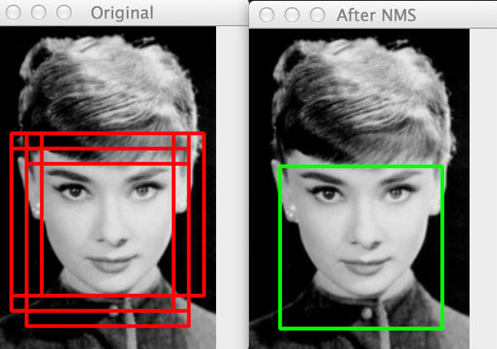
\includegraphics[scale=.3]{images/nms}
  \caption{\em Antes y después de NMS. Adaptado de \cite{Rosebrock2014}} 
  \label{fig:nms}
\end{figure}


\section{\textit{Extreme Programming} (XP)}
\label{preliminares:xp}

Es importante presentar antecedente para caracterizar la metodología que hace de base para la adaptación realizada en el presente trabajo. Extreme Programming consiste, en palabras de su autor, \cite{Beck1999}, a través de su libro \textit{``Extreme Programming Explained: Embrace Change''} en ``una disciplina del negocio de desarrollo de software que enfoca a todo el equipo en metas comunes y alcanzables''. También lo define como ``un estilo de desarrollo de software que se enfoca en una excelente aplicación de técnicas de programación, comunicación clara y trabajo en equipo''. Es, el en fondo, una metodología ágil de desarrollo de software, enfocada principalmente en generar valor agregado a la solución.
El enfoque de XP se centra en ``hacer lo que necesitas hacer para crear valor para el cliente'' \citep{Beck1999}. De esta afirmación se puede desprender que esta metodología se enfoca directamente en el proceso del desarrollo del software, donde ``la programación es la actividad clave''. El espíritu de la metodología es equivalente a conducir un auto (en palabras del autor): no se trata de llevar el auto en la dirección correcta, sino que de poner atención de manera constante y corregir la dirección del auto apenas sea necesario. El desarrollo es guiado a través de cinco valores: comunicación, simplicidad, retroalimentación, valentía y respeto. Para llevar los valores a la práctica, XP se sirve de los principios, que guían las decisiones relativas al proyecto.
\begin{itemize}
\item La retroalimentación: el desarrollo está guiado por pruebas. Cuando se reporta un error en el sistema, debe adjuntarse el caso de prueba fallido. Se postula que el tiempo entre una acción y su retroalimentación debe ser mínimo a fin de poder aprender y realizar cambios si es necesario. Se conversa de manera constante con el cliente, a fin de asegurarse que el producto en desarrollo concuerda con la idea en mente que tiene el cliente de éste y sus expectativas, toda vez que se asume que el cliente no tiene – desde un principio – un concepto absolutamente claro y entendible de lo que necesita, esto es, el equipo de desarrollo no podrá diseñar exactamente lo que el cliente imagina sin su constante retroalimentación sobre el producto que se está elaborando.
\item La simplicidad: para todo problema su solución es extremadamente simple. El código debe diseñarse de tal forma que sea lo más simple posible.
\item La aceptación del cambio: no debe verse al cambio como un elemento a evitar, tendiendo a programar todo con el fin de hacerlo reusable. Si el cliente necesita cambios en el producto en desarrollo, el equipo debe estar dispuesto a asumirlos de manera activa con el fin de poder implementarlos lo más pronto posible.
\end{itemize}
 
Al ser una metodología ágil, XP se orienta más hacia el cambio constante que a una planificación previa extensa y posteriormente inflexible. Beck afirma en su libro que XP puede funcionar con equipos de cualquier tamaño, no obstante cuando fue diseñado su enfoque estaba orientado hacia equipos de tamaño pequeño de no más de diez personas, evolucionando desde su aplicación en desarrollos internos y de menor categoría a ser la metodología principal de desarrollo del software.
XP se centra en llevar al extremo aquello que es considerado bueno, de ahí la razón de ser de la palabra ``extrema'' para el nombre de la metodología. Alienta al lanzamiento frecuente de \textit{releases}, en términos de horas, no en semanas o meses. Establece que el proceso de desarrollo debe hacerse en pares, donde una persona programa y la otra le asiste, revisando aquello que está siendo programado y contribuyendo con ideas. Estos puestos son periódicamente intercambiables. Todos los involucrados deben probar el producto de manera constante: si se detecta una falla, el reporte del problema involucra adjuntar el caso de prueba fallido. Estos \textit{releases} deben ser pequeños incrementos, cuidando además de integrar continuamente. Para que el desarrollo del software cumpla con el valor de la comunicación, el equipo de desarrollo debe definir estándares de programación que sean entendibles por todos: el individualismo y la idiosincrasia de distintos estilos de programación no contribuye al beneficio del grupo, es sólo la manifestación de un estilo individual, que dificulta la comunicación entre los integrantes del equipo al no existir una estructura y estilos comunes de desarrollo del código que puedan ser entendibles rápidamente por todo el equipo. Debe pensarse que todo el equipo es propietario del código que está en desarrollo, por lo tanto, las parejas que están programando una funcionalidad pueden, en teoría, pasar a trabajar rápidamente en otra funcionalidad sin tener que demorarse demasiado en interpretar cuál fue la forma en que se implementó tal funcionalidad por parte de la pareja anterior, por lo tanto, el desarrollo de las funcionalidades se vuelve independiente del programador, sobre todo, del que la haya implementado en primer lugar.
Beck señala que los elementos que diferencian a XP de otras metodologías son.
\begin{itemize}
\item Sus ciclos de desarrollo cortos, que dan como resultado una retroalimentación temprana, concreta y continua.
\item Su aproximación desde la planificación incremental, que rápidamente deriva en un plan general que se espera que evolucione a lo largo de la vida del proyecto.
\item Su habilidad para programar de manera flexible la implementación de funcionalidades, respondiendo a las necesidades cambiantes del negocio.
\item Su dependencia en:
\subitem - Pruebas automatizadas escritas por programadores, clientes y probadores para monitorear el progreso del desarrollo, permitir la evolución del sistema y detectar defectos de manera temprana.
\subitem - La comunicación oral, pruebas y el código fuente para comunicar la estructura e intención del sistema.
\subitem Un proceso de diseño evolutivo que dura tanto como dure el sistema.
\subitem - La colaboración cercana de personas comprometidas con talento común y corriente.
\subitem - Prácticas que funcionan tanto con los instintos a corto plazo de los miembros del equipo y los intereses a largo plazo del proyecto. 
\end{itemize}


\section{Conclusiones del capítulo}
\label{preliminares:conclusiones}

% ***SAV falta ***DQ Revisado

El marco teórico expuesto pretende contextualizar al lector sobre los tópicos más importantes tratados en el presente trabajo de título. Se trata tanto conceptos generales (Visión por computador, Características, Clasificadores) como específicos (SVM, NMS, Adaboost). El conocimiento de estos conceptos y mejor su aplicación por parte del lector facilitará la comprensión del los puntos desarrollados en los capítulos sucesivos. Si fuera necesario obtener mayor información de los conceptos aquí expuestos revisar las referencias citadas, cuyo detalle se encuentra al final del cuerpo principal del presente documento. 

Un resumen breve de los puntos tratados en este capítulo es el que sigue. En primer lugar, se ha revisado el concepto de visión por computador, que es el área general en la que este trabajo se enfoca y que consiste en palabras simples de emular el sentido de la percepción visual de los seres vivos a través de un computador, permitiendo gracias a esto, detectar elementos de interés dentro de imágenes. También se caracterizó el conjunto de datos utilizado por los clasificadores a fin de medir la calidad de sus detecciones; siendo este conjunto único para todos estos clasificadores. Posteriormente se ha detallado cómo las características de los objetos son extraídas de la imágenes a través de algoritmos denominados, descriptores. Se menciona además a los clasificadores los cuales evaluarán la información obtenida en por los descriptores con el objetivo de asignar una clase o categoría, en este caso peatón o no peatón. Posteriormente se trata el método de \textit{Non-maximal supression} que permitió realizar el procesamiento de las imágenes ya clasificadas. Y por último, se ha hecho referencia a \textit{Extreme Programming}, que corresponde a la metodología de desarrollo de software con la que se implementará la solución al problema propuesto.





%--------Métricas
%--------Daniel Quinteros Céspedes
%--------23-09-2014

\chapter{M\'etricas de sensibilidad espacial}
\label{cap:metricas}

Recordando al lector que el presente trabajo de título tiene por objetivo principal realizar un análisis comparativo en base a la sensibilidad espacial de los clasificadores, es necesario definir que es lo que se entiende por sensibilidad espacial y como esto se aplica a este proyecto. Previo a indicar como se concibe la sensibilidad espacial, es necesario tener en consideración que la detección en este trabajo se realiza utilizando una ventana deslizante de clasificación la cual se desplaza por la imagen comprobando la existencia o inexistencia de un peatón en cada punto. 
Teniendo en cuenta lo anterior, la sensibilidad espacial corresponde a la variación de la salida del clasificador cuando la ventana de detección se desplaza por la imagen, en particular se busca analizar este comportamiento en la vecindad del objeto que se desea detectar. Con esto podemos decir que un clasificador con una sensibilidad espacial alta está mejor ``sintonizado'', que uno que posee una baja sensibilidad espacial. A continuación se extenderá un poco esta definición, se presentarán las métricas propuestas y se desarrollará el concepto detrás de la métrica escogida para realizar el análisis comparativo.

\section{Sensibilidad espacial}
\label{metricas:sensibilidad}

Es de esperar que la respuesta de un clasificador indique la pertenencia o no de un objeto a una clase determinada, sin embargo no es la única información que nos 
entrega. Como se mencionó en el capítulo anterior algunos clasificadores toman su decisión utilizando una función de probabilidad condicional por lo que es posible conocer la probabilidad con la que el clasificador afirma la pertenencia a una clase determinada. Por otra parte la salida un clasificador como el SVM lineal representa la distancia del punto evaluado al margen del hiperplano separador. El signo de esta distancia indica su pertenencia o no a la clase. Sin embargo, es razonable pensar que mientras mayor sea la distancia al mencionado hiperplano más clara es su pertenencia o no (dependiendo del signo) a una determinada clase. Estos ejemplos pretenden ilustrar que es posible extraer del clasificador información sobre la confianza con la que afirma su clasificación. 

\begin{figure}[tp]
  \centering
  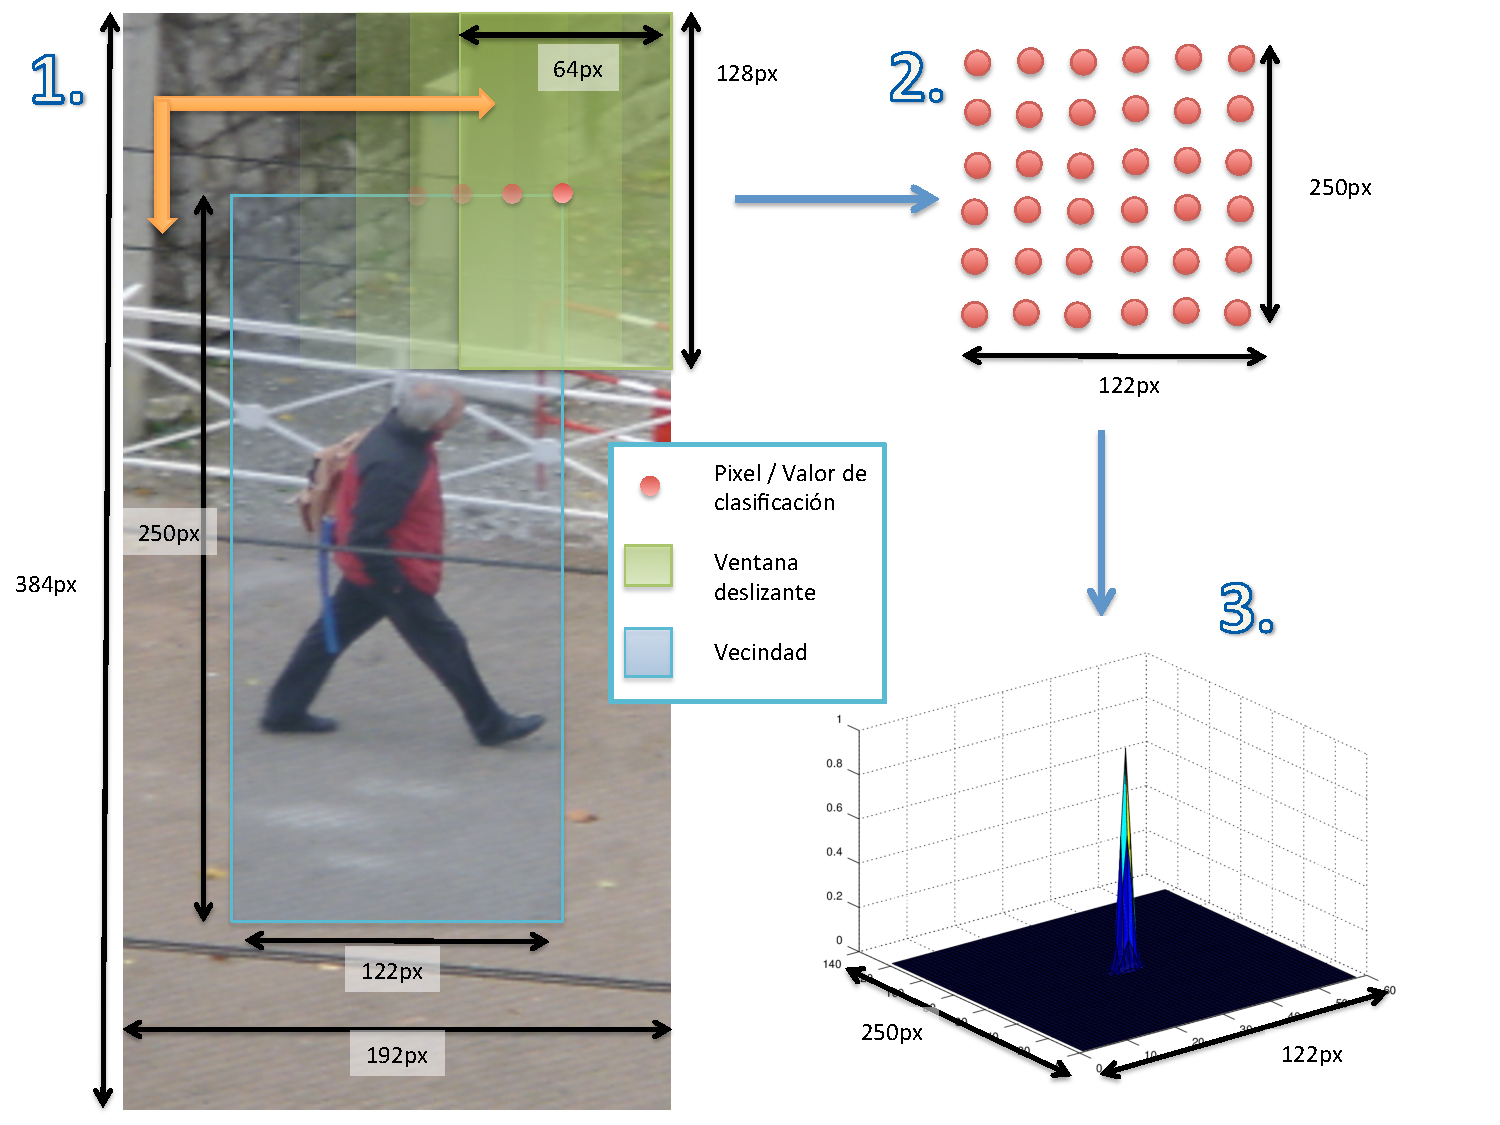
\includegraphics[scale=.6]{images/expected}
  \caption{\em Esquema de Proceso y Resultado esperado.}  
  \label{fig:expected}
\end{figure}

Por otra parte es esperable que un clasificador correctamente sintonizado (con un alta sensibilidad espacial) tenga una salida con mayor índice de confianza mientras la ventana de clasificación se encuentre más cerca del objeto a detectar y aun mucho mayor cuando se encuentre totalmente frente a este. Para comprender más fácilmente este efecto podemos observar en la fig~\ref{fig:expected} un esquema muy general del proceso por el cual se obtienen los resultados y cuales deberían ser los resultados esperados, en primer lugar se encuentra la ventana deslizante que realiza la detección píxel a píxel buscando un peatón en la imagen, luego los valores obtenidos son recogidos en una matriz y evaluados para obtener su gráfico el cual presenta el resultado esperado. Dado que la persona se encuentra en el centro de la imagen es de esperar que en esa zona la confianza de la decisión del clasificador sea mucho más alta que para el resto de la imagen y en un escenario teórico ideal esperamos que la respuesta sea un único impulso en el centro de la imagen analizada pues esto simplificaría de forma considerable el post-procesamiento.


\section{M\'etricas propuestas}
\label{metricas:propuestas}

La \cite{IEEE1990} define un métrica como ``Una medida cuantitativa del grado en que un sistema, componente o proceso posee un atributo dado'', por lo tanto el objetivo de la métrica debe ser en este caso particular definir el grado de sensibilidad espacial que poseen un clasificador para la detección de personas.

\subsection{Curtosis y Asimetría}
\label{propuestas:kys}

Inicialmente se consideró la utilización de una extensión a dos dimensiones de dos medidas que se utilizan en estadística y permitirían describir la sensibilidad espacial, estas son la curtosis (\textit{kurtosis}) y la asimetría (\textit{skewness}). Estas medidas aplicadas sobre los datos obtenidos entregan una descripción de la forma de la distribución. En el caso de la curtosis, mientras mayor sea su valor, la respuesta del clasificador representaría una concentración mayor de datos cercanos a la media, que coexisten con una frecuencia relativamente elevada de datos alejado de ésta. Por otro lado, la asimetría indicará cuán desplazada se encuentra la distribución de un centro de referencia simétrico. Específicamente la curtosis se mide utilizando el coeficiente de curtosis el cual tiene valor 3 cuando la distribución es de tipo normal o mesocúrtica, si el valor es mayor a 3 se conoce como distribución leptocúrtica y si el valor es menor que 3 la distribución es platicúrtica. En la figura~\ref{fig:curtosis} se puede observar de forma gráfica el fenómeno de la curtosis. 

\begin{figure}[tp]
  \centering
  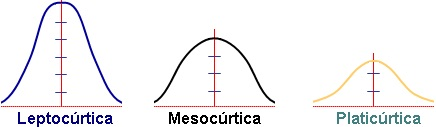
\includegraphics[scale=.6]{images/curtosis}
  \caption{\em Tipos de distribución según su valor de curtosis.}  
  \label{fig:curtosis}
\end{figure}

La asimetría se puede medir con el coeficiente de asimetría de Fisher. Cuando este coeficiente toma valores negativos la distribución es asimétrica negativa o está desplazada a la izquierda, mientras que si el valor es positivo, la distribución es asimétrica positiva y está desplazada a la derecha. En el caso de que la distribución sea simétrica, el valor del coeficiente es cero, sin embargo, el caso contrario no es siempre correcto. El desplazamiento de la asimetría se puede observar gráficamente en la figura~\ref{fig:asimetria}. 

\begin{figure}[tp]
  \centering
  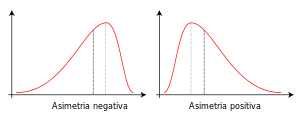
\includegraphics[scale=.6]{images/asimetria}
  \caption{\em Tipos de distribución según su valor de asimetría.}  
  \label{fig:asimetria}
\end{figure}

Estas medidas son muy útiles al trabajar con datos en una dimensión. Sin embargo al realizar una extensión de este procedimiento a dos dimensiones los resultados no fueron los esperados, por lo que fueron reemplazadas por un método más directo que permitiría determinar cuán malo es el valor de la sensibilidad espacial respecto de un modelo dado.

\subsection{Promedio ponderado de las diferencias (PPD)}

\begin{figure}[tp]
  \centering
  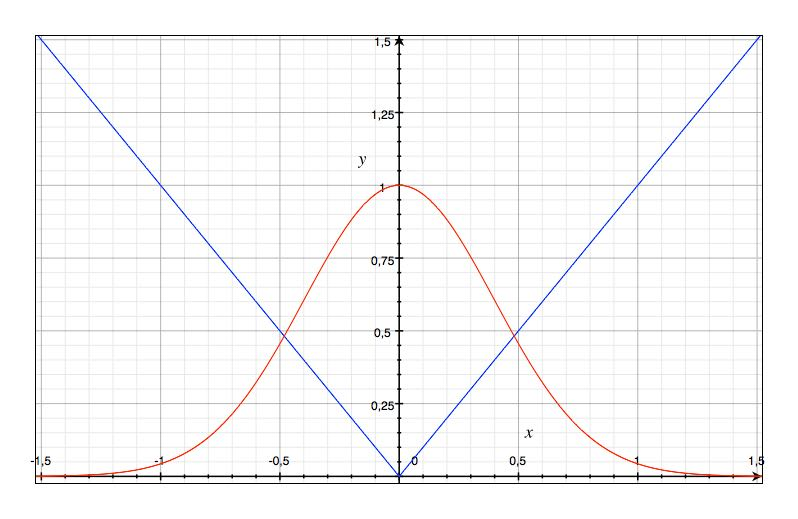
\includegraphics[scale=.4]{images/grafico_ppd}
  \caption{\em Representación de las funciones utilizadas para el cálculo del PPD.}  
  \label{fig:ppd}
\end{figure}

Dadas las dificultades encontradas utilizando la curtosis y la asimetría se hace necesario plantear un nuevo modelo de métrica que  permita describir de mejor forma la sensibilidad espacial. El nuevo modelo de sensibilidad espacial esta inspirado en una distribución normal, dado que en la práctica la probabilidad de obtener un resultado como un impulso es muy baja, por lo que el modelo normal se ajusta mejor a la realidad del fenómeno. La métrica propuesta evalúa el valor absoluto de las diferencias punto a punto de la matriz resultado respecto del modelo de distribución normal en tres dimensiones, luego realiza un promedio ponderado por una función cónica. En la figura~\ref{fig:ppd} se puede observar la abstracción del modelo en dos dimensiones. Es importante señalar que el set de datos se adaptó con una transformación en la cual se situó a la persona a detectar en el centro de la imagen de cada imagen de test y se estandarizó el tamaño de todas estas imágenes. De esta forma se puede comparar en mejor forma distintas combinaciones de descriptor/clasificador.

\begin{figure}[H]
  \centering
  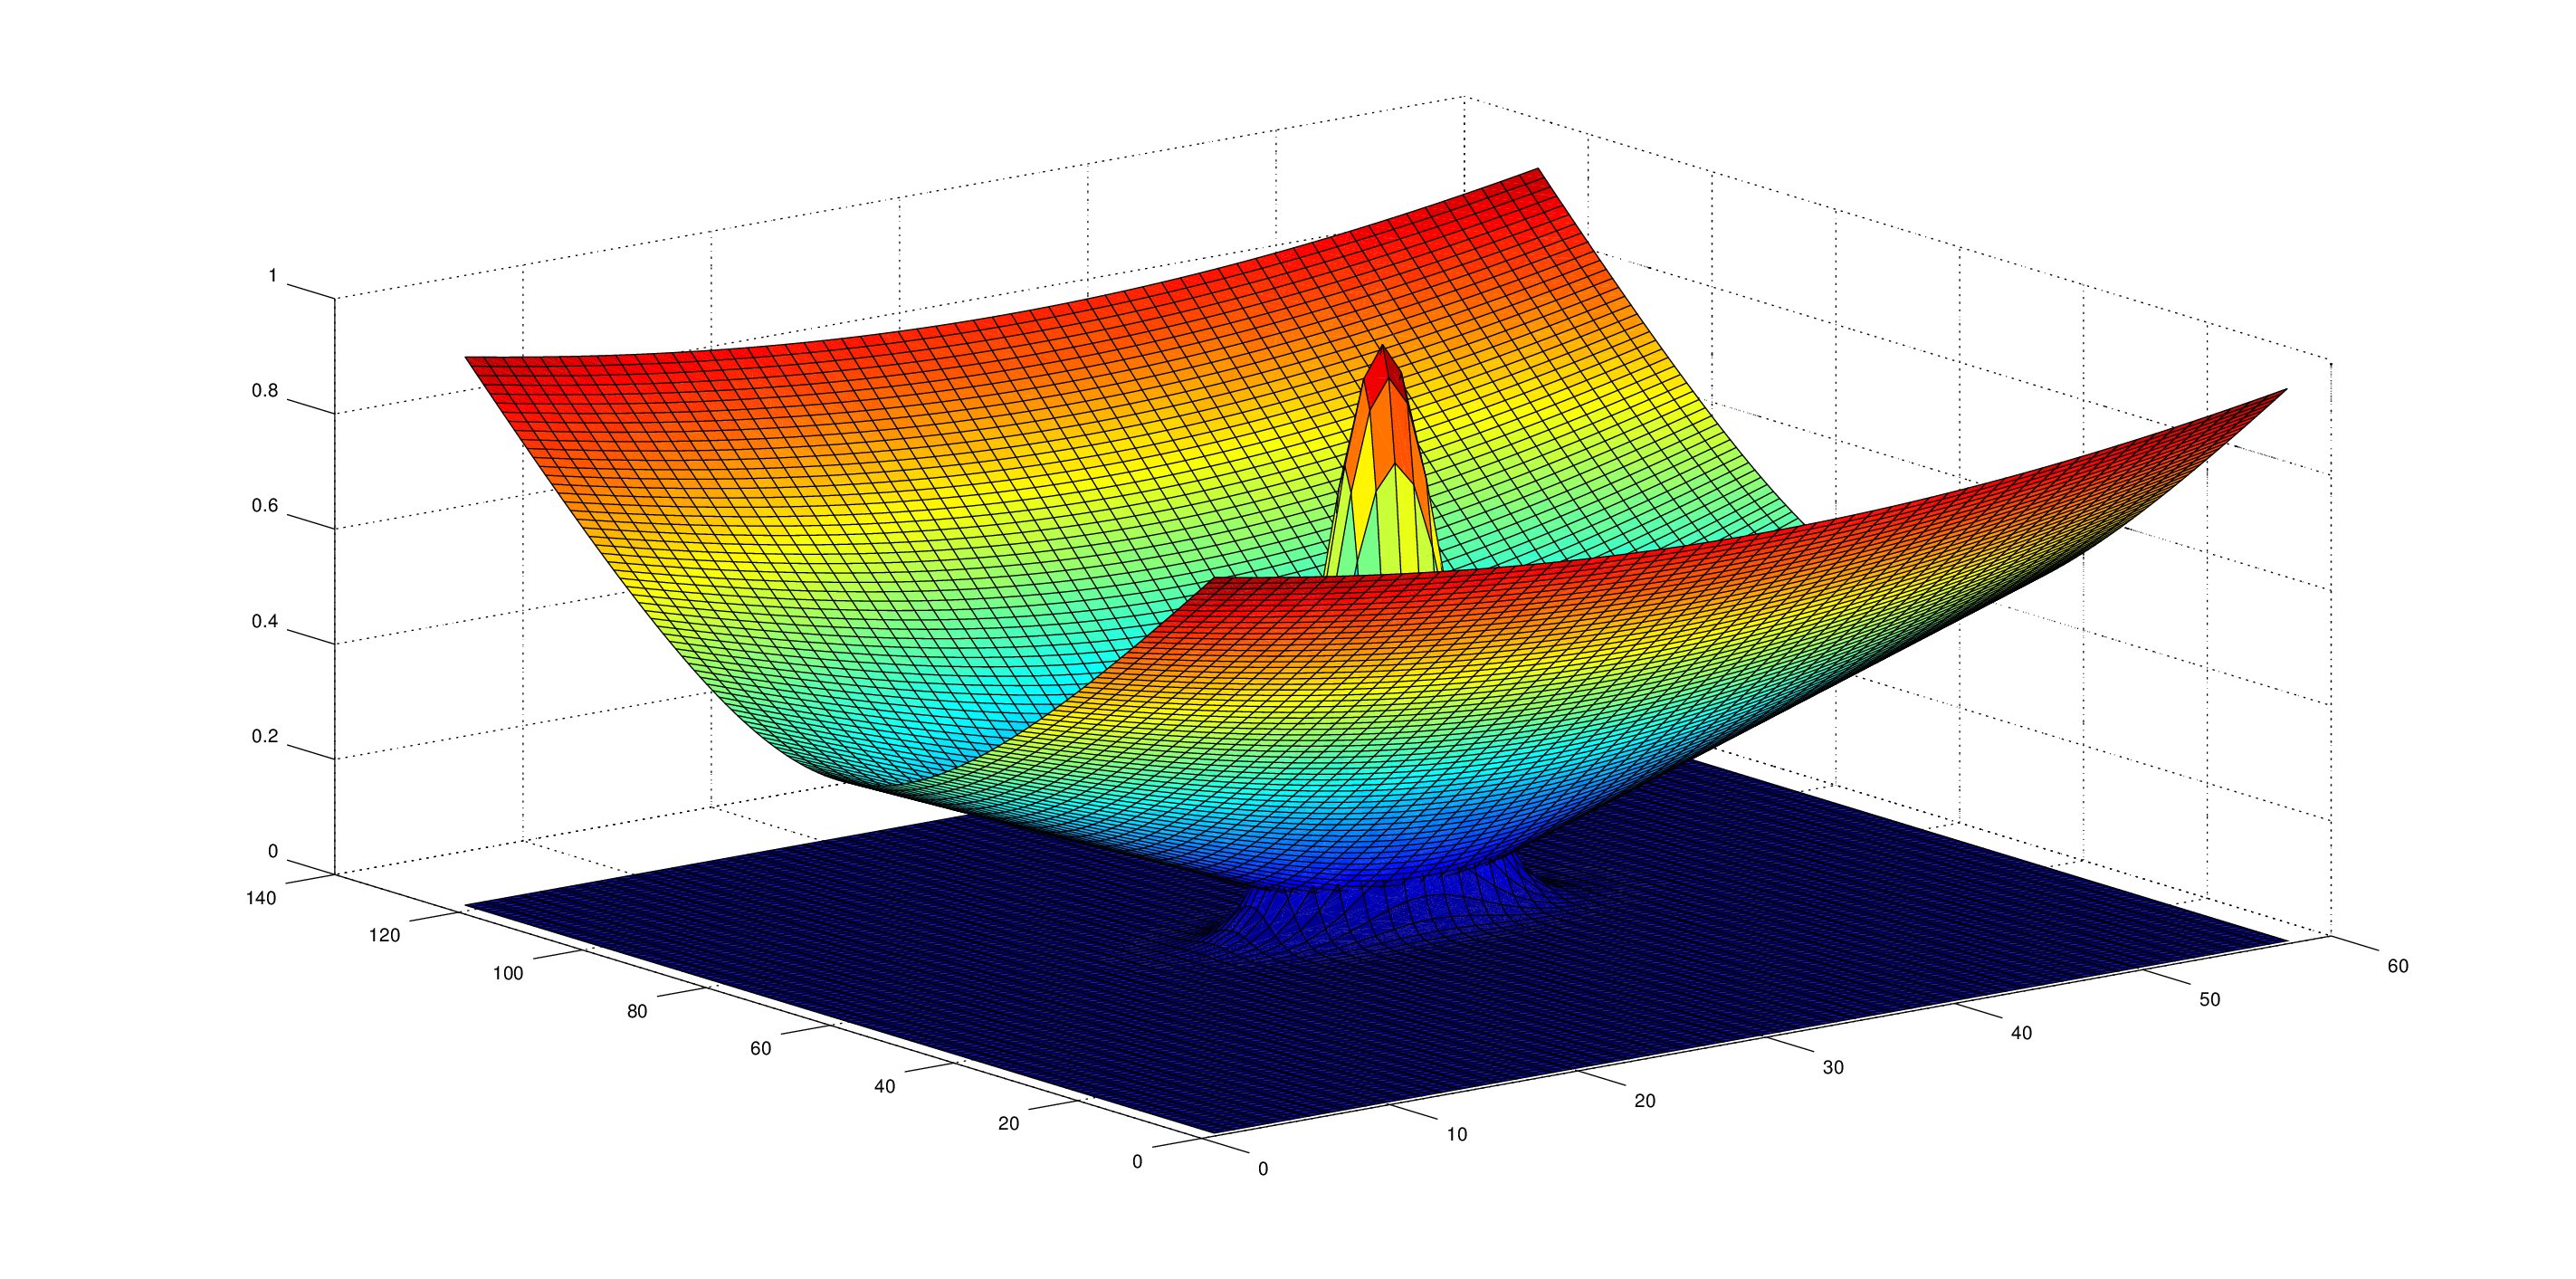
\includegraphics[scale=.3]{images/metrica}
  \caption{\em Representación en tres dimensiones de las funciones utilizadas para el cálculo del PPD.}  
  \label{fig:ppd3d}
\end{figure}

El modelo en tres dimensiones de la métrica es difícil de visualizar por la diferencia de tamaño entre la función cónica y la función normal, sin embargo, en la figura~\ref{fig:ppd3d} se realizó un ajuste de la escala para poder visualizar el efecto.

\subsubsection{Demostración matemática}
\label{sec:dem}

Para demostrar que la función aplicada PPD es efectivamente una métrica es necesario demostrar matemáticamente que cumple con las condiciones para serlo. A continuación se presenta la definición matemática de métrica y la demostración de que PPD cumple con dicha definición

Sea \textit{X} un conjunto. Una función \(d:X\times X\rightarrow \mathbb{R}\) se llama \textit{distancia o métrica} sobre \textit{X} si se cumplen los axiomas de métrica.

\begin{enumerate}
\item \(d(x,y)\geq\)~0
\item \(d(x,y) = \)~0~\(\Leftrightarrow x=y\)
\item \(d(x,y)=d(y,x)\)
\item \(d(x,z)\geq~d(x,y)+d(y,z)\)
\end{enumerate}

Luego de definir una métrica se da paso a la demostración. Sea \(z(x,y)\) la función resultado. Sea \(w(x,y)\) la función modelo. Sea \(c(x,y)\) la función cónica. Donde \(x = 0,1,...,m-1\) e \(y = 0,1,...,n-1\). Entonces la ponderación de la función resultado y modelo con la cónica se puede escribir como.

% ***SAV creo que es mejor no usar * (se confunde con otro operador como convolución) ***DQ Revisado

\begin{enumerate}
\item \(f(x,y) = z(x,y)\ c(x,y) = v_{k}\)
\item \(g(x,y) = w(x,y)\ c(x,y) = u_{k}\)
\end{enumerate}

Donde \(k = 0, 1, 2, ..., mn-1.\) la métrica propuesta queda definida por la expresión~\ref{eq:met}.

\begin{equation}
\centering
\label{eq:met}
 d(u_{k},v_{k})=\sum_{k=0}^{mn-1} \left | u_{k}- v_{k}\right |
\end{equation}

Evaluando los axiomas:
 

\begin{enumerate}
\item \(como \left | u_{k}- v_{k}\right | \geq~0 \forall~k \in~[0,nm-1)] \\ entonces  \sum_{k=0}^{m\ n-1} \left | u_{k}- v_{k}\right | \\ \therefore~d(u_{k},v_{k})\geq~0\)

\item \(d(u_{k},v_{k}) = 0 \\ \Rightarrow \sum_{k=0}^{mn-1} \left | u_{k}- v_{k}\right | = 0 \\ \Rightarrow  \left | u_{k}- v_{k}\right | = 0 \forall~k \in~[0,nm-1] \\ \Rightarrow  u_{k}- v_{k} = 0 \forall~k \in~[0,nm-1] \\ \Rightarrow  u_{k} = v_{k} \)

\item \(d(u_{k},v_{k})=\sum_{k=0}^{mn-1} \left | u_{k}- v_{k}\right | = \sum_{k=0}^{mn-1} \left | v_{k}- u_{k}\right | =  d(v_{k},u_{k}) \)

\item \( d(u_{k},s_{k})=\sum_{k=0}^{mn-1} \left | u_{k} - s_{k}\right | \\
\sum_{k=0}^{mn-1} \left | u_{k} - s_{k}\right | \leq \sum_{k=0}^{mn-1} \left | u_{k} - v_{k}\right | + \left | v_{k} - s_{k}\right | \\
= \sum_{k=0}^{mn-1} \left | u_{k} - v_{k}\right | + \sum_{k=0}^{mn-1} \left | v_{k} - s_{k}\right | \\
= d(u_{k},v_{k}) + d(v_{k},s_{k}) \)

\end{enumerate}


Una vez realizada la demostración las métricas consideras deben ser evaluadas para comprobar su correcto funcionamiento. 

\section{Evaluaci\'on preliminar de las m\'etricas propuestas}
\label{metricas:evaluacion}



\begin{figure}[H]
  \centering
  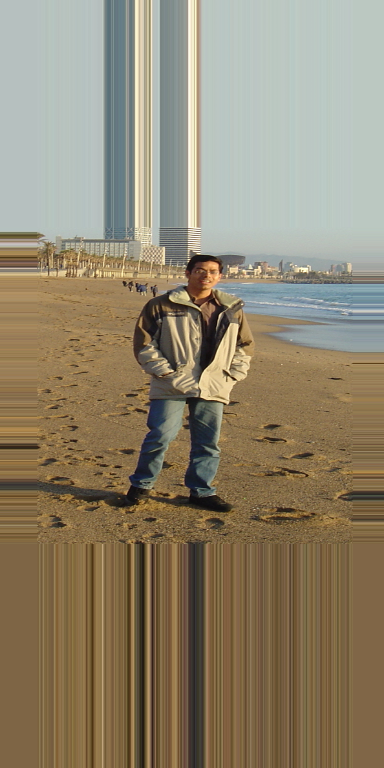
\includegraphics[scale=.25]{images/test1}
  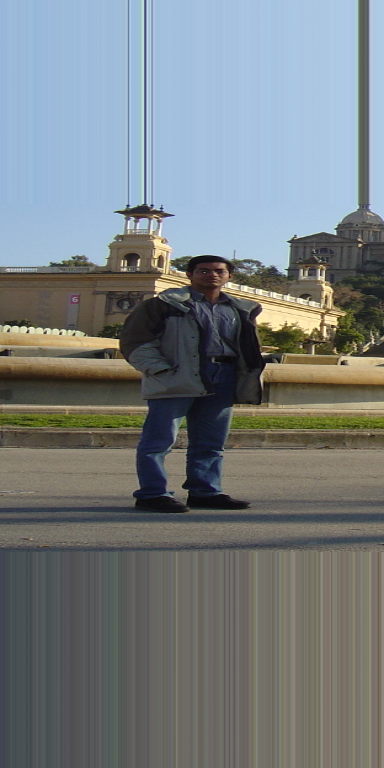
\includegraphics[scale=.25]{images/test2}
  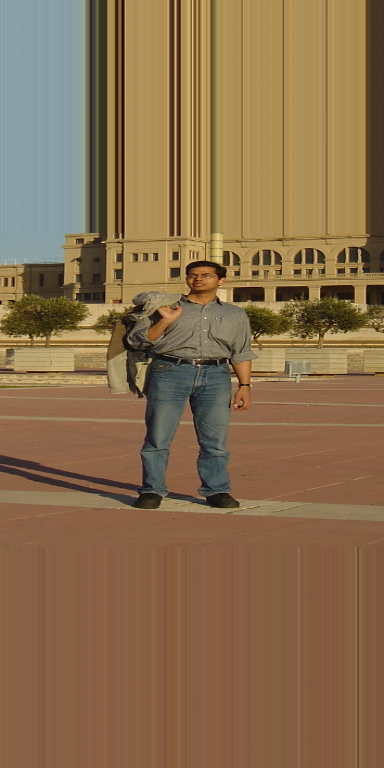
\includegraphics[scale=.25]{images/test3}
  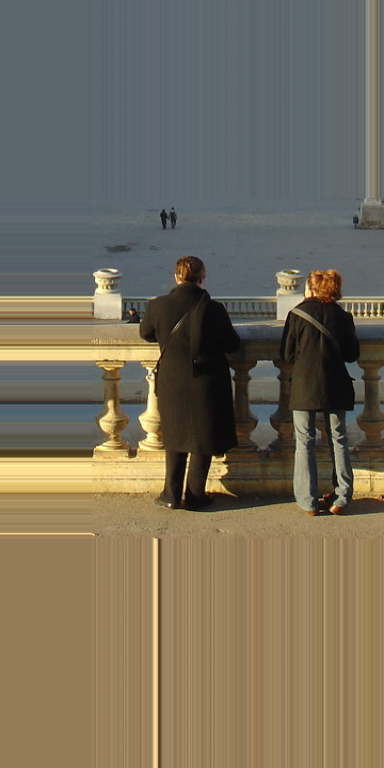
\includegraphics[scale=.25]{images/test4}
  \caption{\em Imágenes utilizadas en la evaluación preliminar, de izquierda a derecha test1.png, test2.png, test3.png, test4.png.}  
  \label{fig:testpersons}
\end{figure}

Una vez propuestas la métricas es necesario evaluar su contingencia respecto del problema de la sensibilidad espacial. Con este fin se desarrolló un software ejemplo preliminar que permite obtener una matriz resultado con valores correspondientes al grado de seguridad con la que un clasificador indica la existencia de un peatón alrededor del \textit{ground truth}. Para  esto se utilizó la implementación del detector utilizando HOG el cual está incluido dentro de la biblioteca OpenCV. Además se consideró como \textit{ground truth} el punto indicado en las anotaciones realizadas por Dalal que acompañan la descarga del set de datos INRIA. 
% ***SAV sería bueno poner una imagen ilustrando esto mostrando el peatón y la vecindad de análisis
Las imágenes utilizadas para realizar la evaluación preliminar fueron extraídas desde el mismo set de datos que finalmente sería utilizado para realizar el análisis comparativo. En la figura~\ref{fig:testpersons} se pueden revisar las imágenes utilizadas.

\begin{figure}[H]
  \centering
  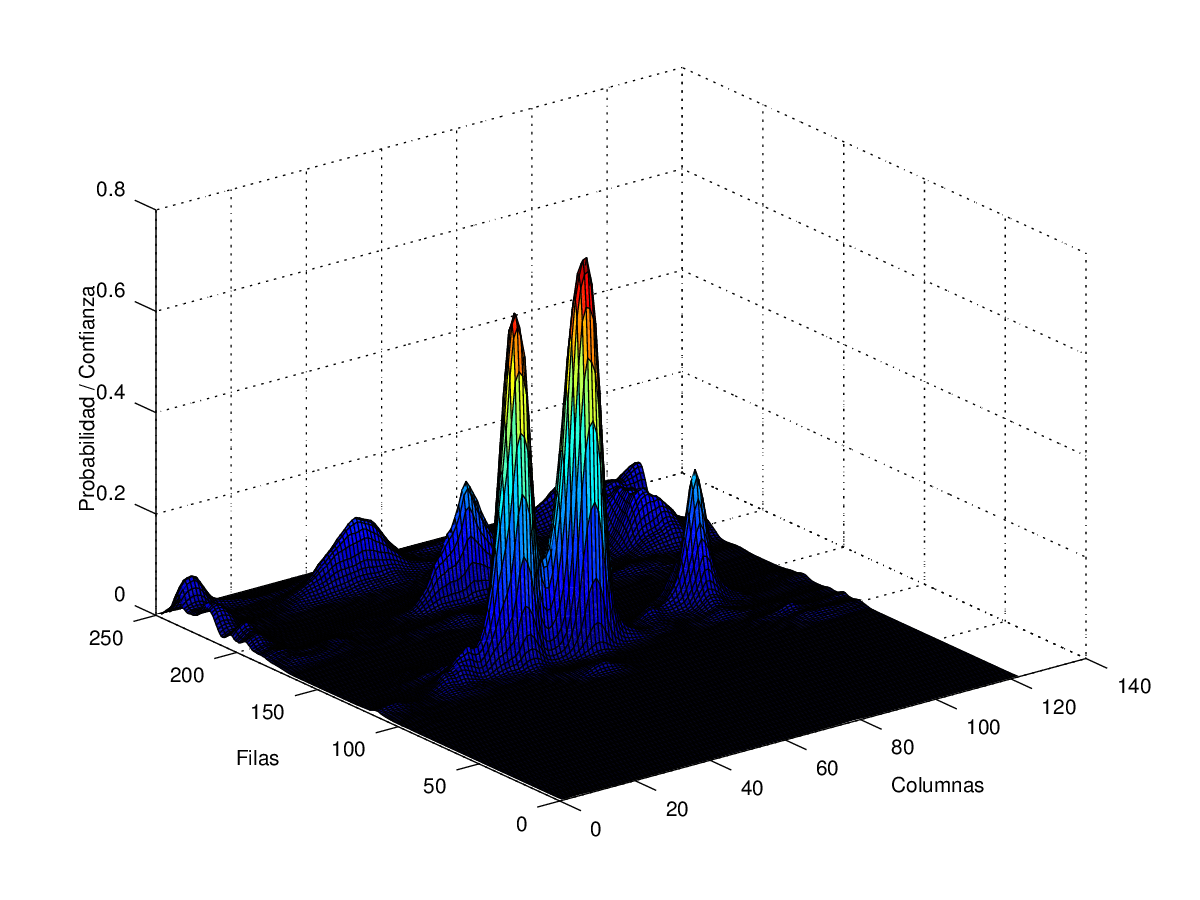
\includegraphics[scale=.6]{images/resultado_ejemplo}
  \caption{\em Resultado obtenido luego de realizar una clasificación exhaustiva de ``test1.png''}  
  \label{fig:ejemploresultado}
\end{figure}

% ***SAV son realmente 3 dimensiones? En el caso estandar es una dimension (por ejemplo el tiempo o una distancia lineal, y la "segunda" dimension es la respuesta). En ls imagenes son dos dimensiones x y más la respuesta. O sea la respuesta es una funcion de 2 dimensiones (x y). *** DQ revisado, efectivamente son dos dimensiones más la respuesta, solo el gráfico es en tres dimensiones.
Dados los problemas mencionados en la sección~\ref{propuestas:kys} sobre la extensión de las métricas a un espacio de dos dimensiones se realizaron las pruebas preliminares con las métricas de curtosis y asimetría para una dimensión, utilizando las proyecciones para las columnas y las filas. A continuación el proceso se detalla sólo para una de la imágenes (``test1.png'') y los resultados generales obtenidos (la gráfica del proceso completo se pueden encontrar en el Anexo~\ref{cap:gapm}).

\begin{figure}[H]
  \centering
  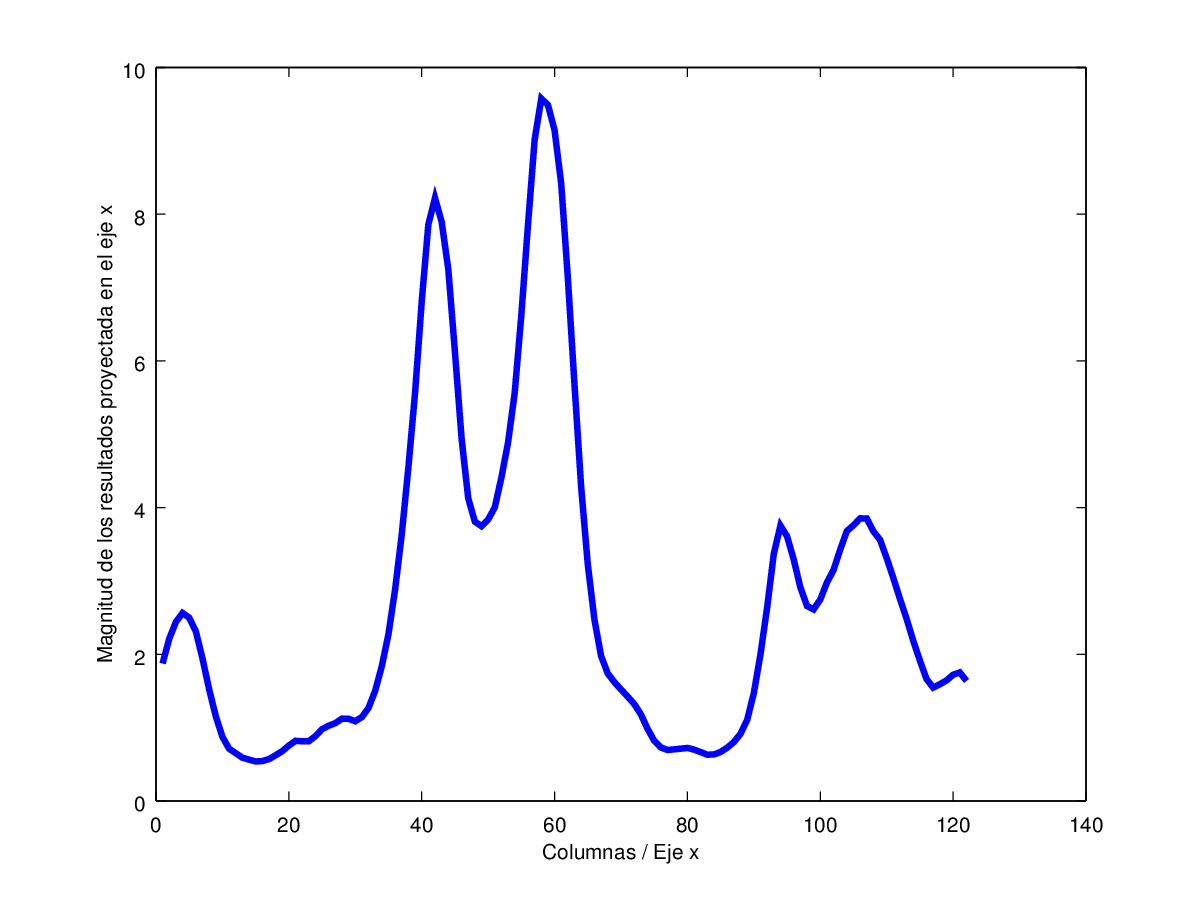
\includegraphics[scale=.35]{images/proyeccionx}
  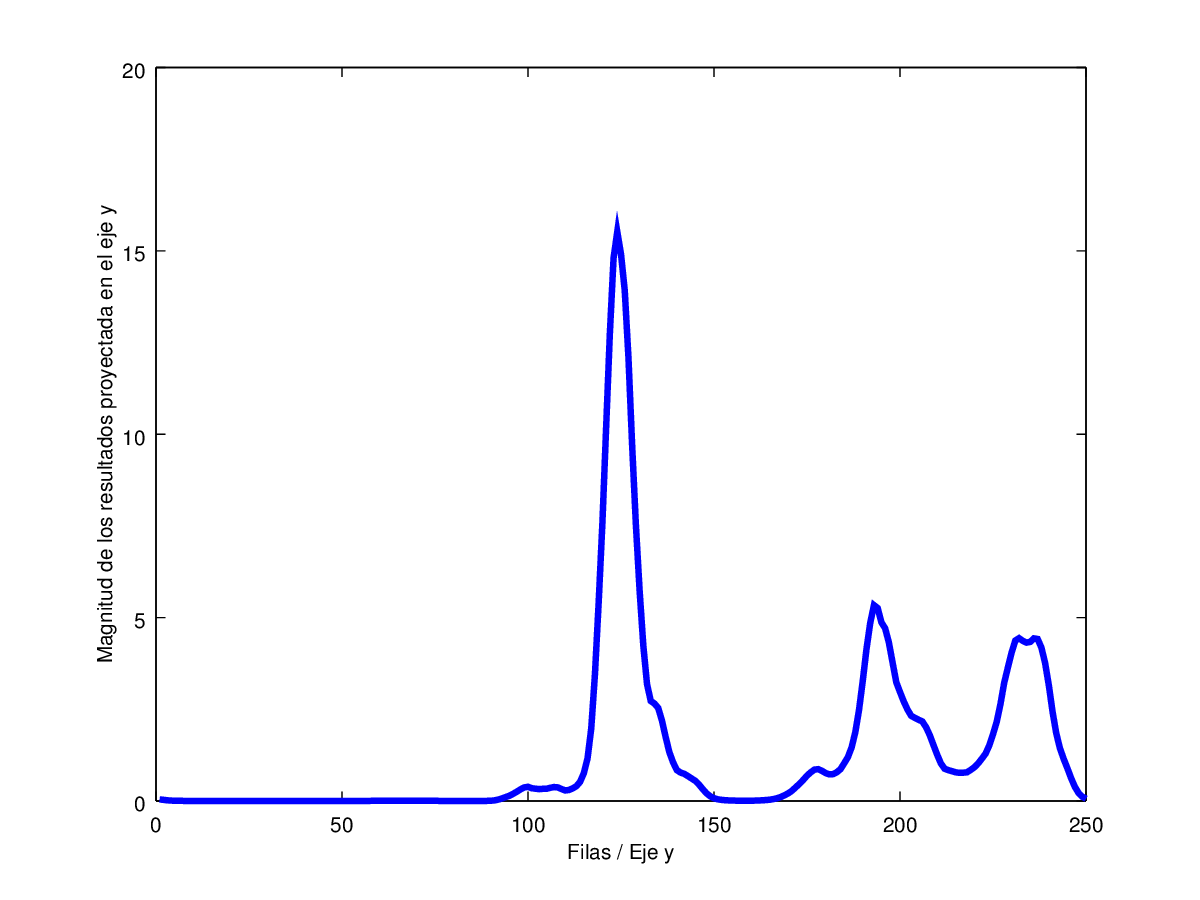
\includegraphics[scale=.35]{images/proyecciony}
  \caption{\em Proyección del resultado para los ejes x (izquierda) e y (derecha).}  
  \label{fig:proyecciones}
\end{figure}

Una vez realizada la clasificación exhaustiva en la imagen se obtiene un resultado como el de la figura~\ref{fig:ejemploresultado}, en este se pueden observar dos elevaciones bastante más pronunciadas que en el resto de la imagen, en la imagen hay solo una persona por lo que sería necesario utilizar NMS (non maxima suppression) para eliminar las detecciones múltiples. Analizaremos la posibilidad de caracterizar esto con la evaluación de la sensibilidad espacial. Para la realización de algunos de los cálculos es necesario obtener las proyecciones para el eje \textit{x} y para el eje \textit{y} las cuales se muestran en la figura~\ref{fig:proyecciones}.

Luego de la proyección, es preciso calcular el centroide y la desviación estándar cuyos valores son requisito previo para el cálculo de la curtosis y la asimetría, finalmente se realizó el cálculo de el PPD, el cual se aplica directamente sobre la matriz sin pasos intermedios, evaluando la diferencia de la matriz en cada punto con el modelo de función y ponderando posteriormente con la función cónica. Así se obtuvieron los resultados para las imágenes analizadas, estos resultados se muestran en la tabla~\ref{tab:resultadospreliminares}. A simple vista se puede comprobar que es posible calcular todas las métricas para todos los ejemplos.

\begin{table}[ht]
\centering
 \caption{\em Resultados obtenidos de la evaluación preliminar.}   \label{tab:resultadospreliminares}
\resizebox{15cm}{!} {
\begin{tabular}{c|c|c|c|c|c|c|c|c|c|}
\cline{2-10}
                                & Centroide x & Centroide y & \begin{tabular}[c]{@{}c@{}}Desviación\\  estándar x\end{tabular} & \begin{tabular}[c]{@{}c@{}}Desviación \\ estándar y\end{tabular} & Asimetría x & Asimetría y & Curtosis x & Curtosis y & PPD    \\ \hline
\multicolumn{1}{|c|}{test1.png} & 61,79       & 167,36      & 30,06                                                            & 46,46                                                            & 0,18        & 0,24        & 2,33       & 1,47       & 0.62338 \\ \hline
\multicolumn{1}{|c|}{test2.png} & 56,74       & 158,8       & 30,26                                                            & 41,74                                                            & 0,3         & 0,49        & 2.51       & 1,86       & 1.39056 \\ \hline
\multicolumn{1}{|c|}{test3.png} & 56,96       & 148,62      & 23,61                                                            & 43,17                                                            & 0,25        & 1,11        & 4,16       & 2,66       & 0.84709 \\ \hline
\multicolumn{1}{|c|}{test4.png} & 66,61       & 131,91      & 27,70                                                            & 40,85                                                            & 0,11        & 1,38        & 2,29       & 3,8        & 0.92963 \\ \hline
\end{tabular}}
\end{table}

Los valores de centroide, desviación estándar, asimetría y curtosis como se mencionó anteriormente son métricas que permiten realizar una descripción de la forma, podemos a través de ellas realizar un breve análisis. Conociendo ambos centroides podemos conocer la posición del centroide en el plano \textit{(x,y)}. Por otra parte la asimetría nos indica hacia donde se encuentra desplazada la distribución de valores, sin embargo no entregan mayor información en cuanto a que tan sensible o no es el comportamiento del clasificador. El PPD si bien no entrega información en detalle de la forma, indica de forma directa un valor representativo de sensibilidad espacial y se acerca mejor al objetivo de realizar una comparación ya que el indicador entrega un valor mayor mientras peor sea la sensibilidad del clasificador. Sin embargo, la métrica tiene algunos puntos ciegos, por ejemplo cuando el valor evaluado es cero el resultado es positivo  como se muestra en la tabla~\ref{tab:planas}. Esto resulta inconveniente para diferenciar de otra repuesta que tenga una diferencia semejante con el modelo planteado, pero en el sentido opuesto.

\begin{table}[h]
\centering
  \caption{\em Evaluación de matrices con valores constantes para todos sus puntos. }   \label{tab:planas}
\begin{tabular}{c|c|}
\cline{2-2}
                                 & PPD    \\ \hline
\multicolumn{1}{|c|}{Matriz 0}   &  0.00000602 \\ \hline
\multicolumn{1}{|c|}{Matriz 0.1} &  0.73720 \\ \hline
\multicolumn{1}{|c|}{Matriz 0.5}  & 36.85977 \\ \hline
\multicolumn{1}{|c|}{Matriz 1}  &  73.71955 \\ \hline
\end{tabular}
\end{table}

Comprobando los resultados de las métricas se puede comprender que estas son complementarias y ambas son útiles, para caracterizar la sensibilidad espacial, sin embargo, dado su perfil comparativo, PPD es la mejor elección para continuar el análisis.

\section{Conclusiones del capítulo}
\label{metricas:conclusiones}

Resumiendo, en este capítulo se ha hablado acerca de las métricas, esto es, de las medidas cuantitativas del grado en que un sistema, componente o proceso posee un atributo dado. Las métricas a las que se hace mención son aquellas establecidas con respecto de la sensibilidad espacial de los clasificadores, esto es, cómo responde el clasificador a medida que la ventana de desplazamiento se va deslizando por la imagen, siendo el caso ideal que el clasificador no detectará ningún objeto válido (en este caso, personas) a menos que ésta se encuentre perfectamente centrada dentro de la ventana de detección, por lo que idealmente no debería detectar a una persona si sólo está contenida parcialmente dentro de la ventana de detección. A través del establecimiento de las métricas se puede determinar de manera concreta qué tan buena es la sensibilidad espacial de determinado clasificador, factor que constituye parte fundamental del presente trabajo. 

La sensibilidad espacial de un clasificador debe ser caracterizada para ayudar a mejorar el problema del post-procesamiento. Sin embargo, es necesario cuantificar este comportamiento; para esto se proponen en total tres métodos, dos de forma (curtosis y asimetría) y una de magnitud (PPD). Estas métricas son complementarias en el análisis y la caracterización de la sensibilidad espacial. Sin embargo, PPD es la mejor alternativa para la prosecución del presente trabajo, dado que permite realizar una comparación directa. Por otra parte, como trabajo futuro, es importante realizar aportes sobre la métricas tanto para mejorarlas como para complementar con otras que permitan un avance en la caracterización completa de la sensibilidad espacial.

En los capítulos siguientes se explicará en detalle el funcionamiento de los descriptores de características y clasificadores utilizados en el proceso.
\chapter{Descriptores y  Clasificadores}
\label{cap:caract}

Tal como fue mencionado en la sección~\ref{preliminares:caract} la extracción de características como parte inicial de un algoritmo de detección de peatones es un proceso que permite describir aspectos relevantes de una imagen o vídeo como por ejemplo, color, textura, movimiento, entre otros. A este conjunto de características obtenidas se le conoce como descriptores. Para obtener estos descriptores existen gran cantidad de algoritmos, es importante entonces caracterizar el descriptor utilizado para el desarrollo del proyecto. A continuación se expone una reseña de algunos de los descriptores que se utilizan para la tarea detección de peatones según \cite{dollar2012}. Luego se indicarán las razones de la utilización del Histograma de Gradientes Orientados (HOG)~\citep{dalal2005} en el desarrollo de este trabajo. Por otra parte se revisará el funcionamiento de otros descriptores en parte teórica y en base a algunos ejemplos. En particular se expondrá breves nociones sobre SURF, propuesto por \cite{Bay2006} y \textit{Haar-like features} utilizadas por una amplia variedad de autores \citep{Papageorgiou2000, viola2001, Lienhart2002}.  

Luego de la extracción de características para determinar la existencia de un peatón en una imagen es necesario realizar un proceso de clasificación es decir serán definidas dos clases: peatón y no peatón.

Los clasificadores son algoritmos que permiten identificar y asignar un elemento que es utilizado de entrada a una categoría determinada. Sin embargo, la salida de un clasificador no es necesariamente solo una etiqueta de la categoría y en muchos casos la salida de un clasificador representa un valor obtenido una operación matemática que se encuentra descrita en el diseño de cada clasificador, los orígenes de los clasificadores son muy diversos por lo cual sus resultados no siempre son comparables.

\section{Descriptores}
\label{caract:descriptores}

Dada la elección de HOG como descriptor, es importante conocer en profundidad su funcionamiento y la forma en que se generan los vectores de características que permitirán entrenar los clasificadores utilizados en el presente trabajo. A continuación una breve introducción de cada uno de los descriptores considerados. 

\subsection{Análisis de descriptores}

\subsubsection{Histograma de gradientes orientados}
\label{descriptores:hog}

\textit{Histogram of Oriented Gradients}~(HOG) en español histograma de gradientes orientados, propuesto por primera vez por \cite{dalal2005}. Es un algoritmo descriptor de características hoy utilizado ampliamente en visión por computador para problemas de detección de objetos y en particular de la detección de personas. Esta técnica permite obtener a partir de una sección de la imagen un vector de características el cual es utilizado por algoritmos de aprendizaje de máquina para realizar una clasificación.

El método tal como fue descrito por \cite{dalal2006} está basado en la evaluación de un rejilla densa de histogramas locales normalizados de las orientaciones de los gradientes de la imagen, esto por que la hipótesis planteada era que la forma y la apariencia de un objeto estaba bien representada por la distribución local de los gradientes o direcciones de los bordes. El algoritmo tiene por estructura una cadena de cinco pasos la cual permite la extracción de este tipo de  características, los que son interesantes de conocer por lo que se explican a continuación .

\begin{itemize}
\item El primer paso es opcional dentro del proceso y consiste en realizar una normalización o ecualización de toda la imagen que tiene por objeto reducir las posible influencia de los efectos producidos por la iluminación.
\item El segundo paso corresponde al cálculo de los gradientes lo que permite describir los bordes en la imagen y también obtener información sobre la textura. Para esto se utiliza el canal de color dominante lo que permite mantener el color lo más invariante posible.
\item En el tercer paso realiza un división de la imagen en pequeños pedazos llamados \textit{``cells''} (celda) y para cada celda se calcula un histograma de gradientes local. La combinación de la información obtenida de estos histogramas locales forma el``histograma de orientación'' básico. Este método esta inspirado en el mismo tipo de características que el utilizado en SIFT \citep{Lowe2004}
\item El cuarto paso realiza una normalización, tomando un grupo de celdas al que se denomina ``bloques'' toma un valor acumulado de los histogramas locales y el resultado se utiliza para normalizar cada celda en el bloque este bloque normaliza es que se conoce como histograma de gradiente orientado.
\item Finalmente los descriptores HOG obtenidos de todos los bloques son combinados en un vector de características que se utilizan con el clasificador.
\end{itemize}

\begin{figure}[tp]
  \centering
  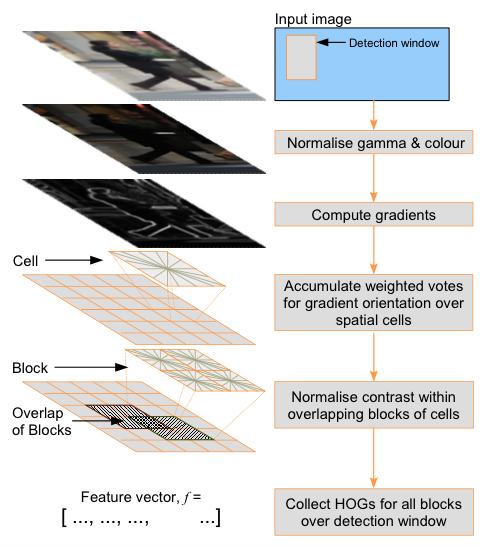
\includegraphics[scale=.6]{images/hogprocess}
  \caption{\em Estructura del proceso general de extracción de características utilizando el algoritmo de extracción HOG. Obtenido de \cite{dalal2006}}  
  \label{fig:hogscheme}
\end{figure}

\subsubsection{\textit{Speeded Up Robust Features} (SURF)}

SURF fue presentado por primera vez por \cite{Bay2006}, este tipo de extractor de características está inspirado en \textit{Scale-invariant feature transform} (SIFT) \citep{Lowe2004}, es un descriptor orientado a la búsqueda de puntos de interés, para realizar esto se realiza una replicación de la imagen en forma piramidal gaussiana o laplaciana con el fin de obtener un efecto borroso llamado \textit{scale-space}, el cual permite obtener puntos de interés que se logran mantener invariantes al variar su escala. 

El principal aporte de SURF es que con el cambio de esquema realizado respecto de SIFT puede mejorar la velocidad de cómputo manteniendo en teoría la calidad de los puntos de interés. El cambio de esquema tiene relación principalmente con que el cálculo con gaussianas realizado en SIFT es reemplazado por aproximaciones cuadradas en SURF. Un ejemplo de los operadores utilizados se muestra en \ref{fig:gaussians}, lo que al realizar la convolución resulta mucho más rápido. Para la búsqueda de los puntos de interés se utiliza un detector de \textit{Binary Large Objects} (BLOB) basado en la matriz Hessiana nombrado \textit{Fast Hessian Detector}.

\begin{figure}[hp]
  \centering
  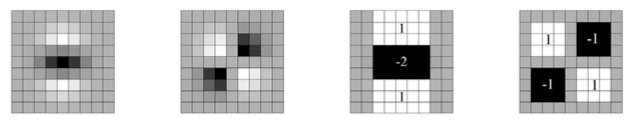
\includegraphics[scale=.6]{images/gaussian}
  \caption{\em Ejemplos de la aproximación de los gaussianas (izquierda) en cuadrados (derecha), los valores grises son cero. Imagen obtenida de \cite{Bay2006} }  
  \label{fig:gaussians}
\end{figure}

Dentro de la documentación de MATLAB, es posible encontrar un ejemplo de funcionamiento de SURF que resulta clarificador para entender lo antes expuesto.

En el ejemplo se muestra un algoritmo para encontrar un objeto especifico basado en puntos clave que se corresponden entre la imagen original y la de referencia, los puntos clave son obtenidos utilizando la implementación en MATLAB del descriptor SURF.

\begin{figure}[hp]
  \centering
  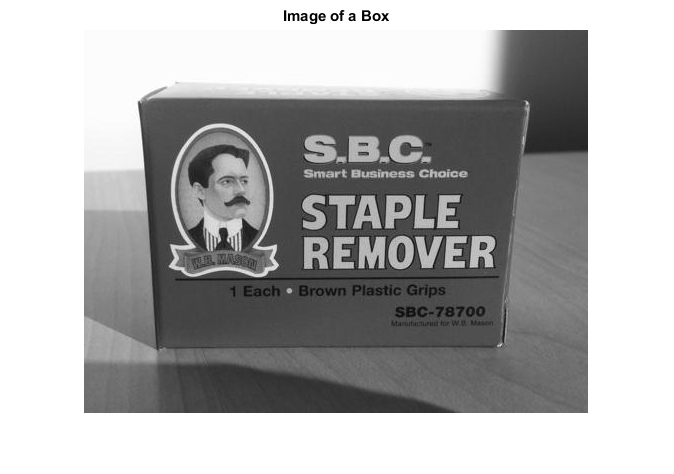
\includegraphics[scale=.4]{images/surfbox}
  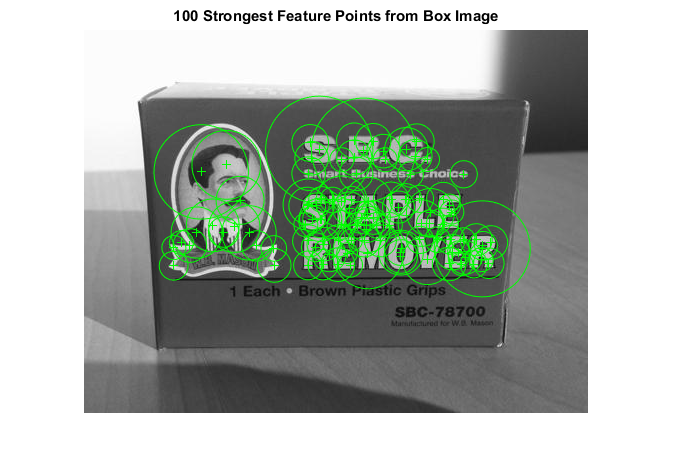
\includegraphics[scale=.4]{images/surfedbox}
  \caption{\em En la imagen, a la izquierda se observa el objeto a detectar, a la derecha el resultado obtenido luego de utilizar el detector \textit{Fast Hessian Detector} como los mostrados en la fig~\ref{fig:gaussians}. Imágenes obtenidas de \cite{matlab2014} }   \label{fig:surfbox}
\end{figure}

\begin{figure}
  \centering
  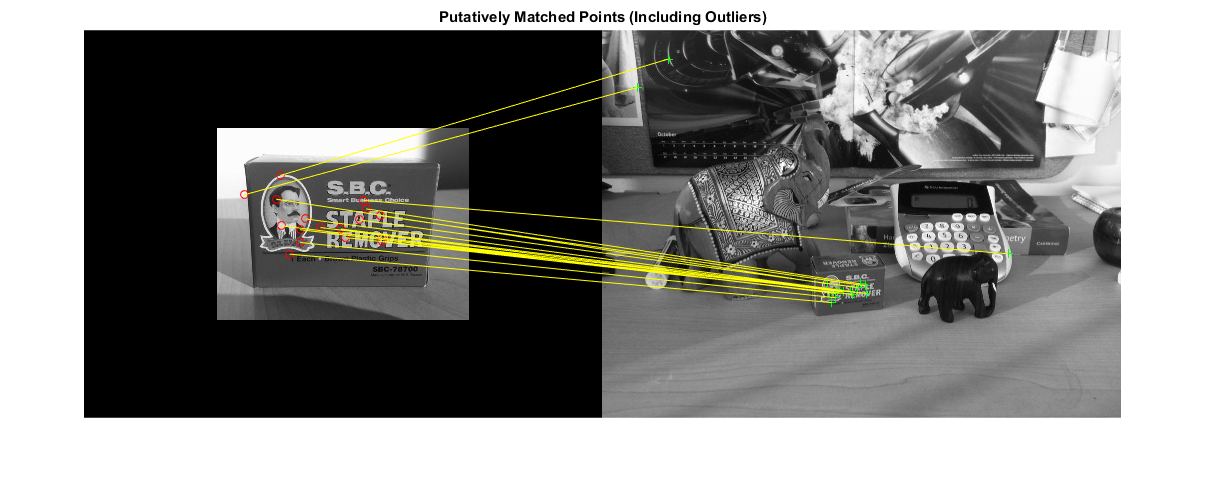
\includegraphics[scale=.4]{images/surfmatching}
  \caption{\em En la imagen. Con los puntos de interés seleccionados se realiza el proceso de búsqueda o \textit{matching}. Imágenes obtenidas de \cite{matlab2014} }   \label{fig:surfmatching}
\end{figure}

\subsubsection{\textit{Haar-like Features}}

La extracción de características de este tipo está orientado a buscar en la imagen la presencia o ausencia de ciertas características en la imagen, como bordes o cambios de textura. En específico \textit{Haar-like Features} considera regiones rectangulares adyacentes en alguna parte de la imagen y calcula la diferencia entre las suma de de las intensidades de cada píxel.

\begin{figure}[hp]
  \centering
  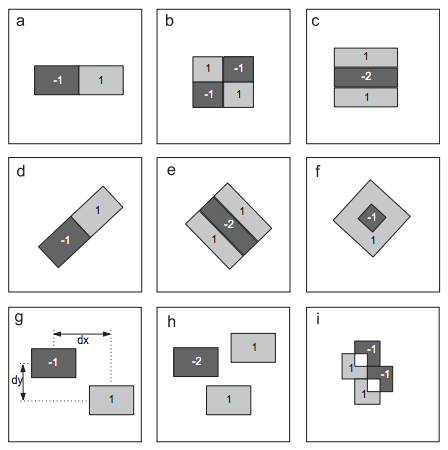
\includegraphics[scale=.3]{images/haarlike}
  \caption{\em Ejemplos \textit{Haar-like Features}. Obtenido de \cite{Pavani2010} }  
  \label{fig:haar}
\end{figure}

\section{Selección del descriptor y proceso de \\extracción de características}
\label{caract:seleccion}

Una vez revisada la información acerca de los descriptores que posiblemente se utilizarían es necesario realizar la selección del descriptor y mencionar las razones para su elección, además el proceso a través del cual se realizó la extracción de características.

\subsection{Selección del descriptor de características}

Se mencionó al inicio de este capítulo (\ref{cap:caract}) y en la sección~\ref{caract:descriptores} un adelanto del resultado sobre el descriptor que finalmente sería escogido para la realización del análisis comparativo. Aquí se ilustran las razones para su elección.

``HOG...es uno de los de los descriptores de características más comúnmente utilizado para la detección de peatones, dada su gran capacidad para describir objetos.'' \citep{Zheng2012}, de esta forma comienzan Zheng y Chen a describir HOG en \textit{``A review on vision-based pedestrian detection''}. HOG es un descriptor realmente popular que se encuentra referenciado en prácticamente cualquier trabajo del área, lo que trae consigo una amplia cantidad de información sobre este. A continuación se enuncian las razones más importante de la elección de HOG.

\begin{itemize}
\item Es un descriptor de características ampliamente referenciado, por lo que hay mucha información sobre él.
\item Se han realizado muchas aplicaciones utilizando HOG, por lo que el impacto de una posible mejoría es mayor.
\item Posee una implementación en OpenCV que es sencilla de utilizar.
\item Dado el grado de importancia conferido tiene respaldo para ser bueno como elemento para realizar pruebas.
\end{itemize}

Algunos de los aspectos negativo de esta elección es la poca variabilidad en cuanto a descriptores, sin embargo esta elección se realizó dada la prioridad otorgada a la evaluación en diferentes escalas, lo que será explicada más adelante.

\subsection{Proceso de extracción de características}
\label{caract:extraccion}

Previo al proceso mismo de extracción de características fue necesario realizar la normalización del conjunto de datos de peatones INRIA de manera que el resultado fuera directamente comparable, para realizar esto se tomaron en cuenta las siguientes consideraciones.

\begin{itemize}
\item Para facilitar la comparación final cada peatón objeto de la detección debe encontrarse en el centro de la imagen. (Esto se cumple por defecto para del conjunto de entrenamiento, mas no para el conjunto de pruebas). 

\item Se considerará en la detección toda la vecindad inmediata del peatón, es decir al comenzar la detección la ventana de clasificación se encontrará apenas fuera por la parte superior e izquierda y al finalizar se encontrará apenas fuera por la parte inferior y derecha.

\item Se considerará que el peatón se encuentra certeramente donde indican las anotaciones, aún cuando existe la certeza de que esto no es perfecto ya que en efecto hay un peatón en cada una de las anotaciones, sin embargo, no está totalmente centrado.

\item Con el fin de analizar la variación de la sensibilidad espacial a diferentes escalas, la evaluación será realizada en cuatro escalas diferentes por lo que es necesario ampliar o reducir cada imagen según sea necesario. 
\end{itemize}

El proceso de extracción de características es directo, ya que la implementación utilizada de HOG se puede encontrar dentro de la biblioteca OpenCV y esta implementación posee la función \textit{getDescriptors} la cual recibe como entrada la imagen y entrega el valor del vector de características HOG estos vectores son recolectados en una matriz de características que luego será utilizada para el entrenamiento de los clasificadores.

\begin{figure}[hp]
  \centering
  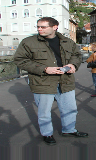
\includegraphics[scale=.6]{images/train1}
  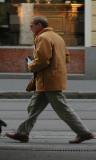
\includegraphics[scale=.6]{images/train2}
  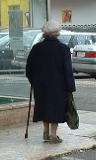
\includegraphics[scale=.6]{images/train3}
  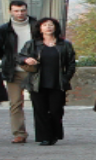
\includegraphics[scale=.6]{images/train4}
  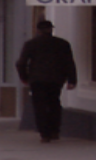
\includegraphics[scale=.6]{images/train5}\\
  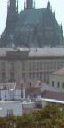
\includegraphics[scale=.9]{images/neg1}
  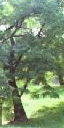
\includegraphics[scale=.9]{images/neg2}
  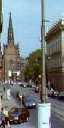
\includegraphics[scale=.9]{images/neg3}
  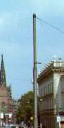
\includegraphics[scale=.9]{images/neg4}
  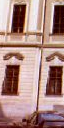
\includegraphics[scale=.9]{images/neg5}
  \caption{\em Imágenes de ejemplo obtenidas del conjunto de entrenamiento del set de datos INRIA, arriba imágenes positivas``clase peatón'', abajo imágenes negativas ´´clase no-peatón'' }  
  \label{fig:trainimgs}
\end{figure}

En la figura~\ref{fig:trainimgs} se observan ejemplos de las imágenes de conjunto de entrenamiento del set de datos INRIA de las cuales se extrae el vector de características. Con el objetivo de comparar la sensibilidad espacial a escalas diferentes se hizo necesario realizar un cambio de tamaño a las imágenes de entrenamiento del set de datos, los tamaños utilizados según la ventana de clasificación (los tamaños reales son levemente superiores para evitar problemas de borde) fueron 32x64px, 64x128px, 128x256px, 256x512px. El tamaño original de la ventana es de 64px de ancho y 128px de alto este tamaño está fijado por defecto en el set de datos, para realizar comparaciones se mantuvo la proporción 1:2, pero se amplió y redujo el tamaño de las imágenes para estudiar el comportamiento del clasificador a diferentes escalas.


\section{Clasificadores}
\label{sec:clasif}
 
Una vez determinado cuál será el descriptor de características utilizado, el siguiente paso es determinar cuáles serán los clasificadores a utilizar. En esta sección se revisarán los clasificadores estudiados, la selección , el entrenamiento y el proceso de normalización de la salida.

\subsection{Clasificadores estudiados}

\subsubsection{SVM}
\label{propuestas:svmlineal}

La implementación utilizada del SVM lineal parte de la biblioteca OpenCV en su módulo de \textit{machine learning}. Esta implementación esta basada en la biblioteca LibSVM \citep{Chang2011}. Dentro del módulo antes mencionado no sólo es posible encontrar una implementación para SVM con un kernel lineal, sino que también para kernel polinomial, radial y sigmoidal.
Para el entrenamiento del SVM se consideraron los parámetros por defecto que se pueden observar en la figura~\ref{fig:svmparams}. 

\begin{figure}[H]
  \centering
  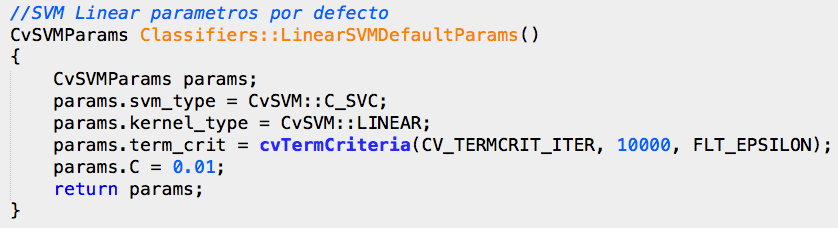
\includegraphics[scale=.6]{images/svmparams}
  \caption{\em Parámetros por defecto de SVM Lineal para la construcción de los diferentes modelos utilizados en el análisis. }  
  \label{fig:svmparams}
\end{figure}

Los modelos utilizados del clasificador SVM lineal se construyeron utilizando los vectores de características obtenidos del set de imágenes positivas para entrenamiento del set de datos INRIA y 10 recortes por imagen del set de entrenamiento con imágenes negativas también del set de datos INRIA.

\subsubsection{Adaboost}
\label{propuestas:adaboost}

Dentro del módulo de \textit{machine learning} de OpenCV es posible encontrar un sub módulo de \textit{boosting} en el cual hay algoritmos como Adaboost discreto y real, LogiBoost, y \textit{Gentle} Adaboost. Esta implementación es propia de OpenCV y está basada teóricamente en la propuestas de \cite{Hastie2005} y \cite{Friedman2000}.


\begin{figure}[H]
  \centering
  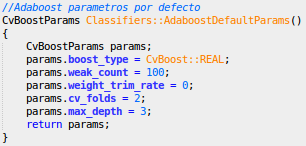
\includegraphics[scale=.6]{images/boostparams}
  \caption{\em Parámetros por defecto de Adaboost Real para la construcción de los diferentes modelos utilizados en el análisis.  }  
  \label{fig:boostparams}
\end{figure}

Al igual que para el SVM lineal se seleccionaron los parámetros por defecto, los que se pueden observar en la figura~\ref{fig:boostparams}; y se construyeron los modelos utilizando los mismos vectores de características (obtenidos con el algoritmo HOG) que se utilizaron para la construcción de los modelos de SVM lineal, con el fin de realizar una comparación.

\section{Selección de clasificadores y entrenamiento}
\label{clasificadores:seleccion}

La selección de clasificadores fue en base a la investigación teórica sin embargo, es conveniente indicar cuáles son la principales razones de seleccionar éstos y no otro tipo de clasificadores. Por otra parte, el proceso de entrenamiento fue exclusivamente tomar procesos ya implementados de OpenCV e incorporarlos en el proceso general. Sin embargo, como será explicado con más detalle en el capítulo~\ref{cap:eval} se realizó otro proceso de entrenamiento relacionado con la función utilizada para normalizar la salidas de los clasificadores.
% ***SAV la frase anterior es difícil de entender, podrías decir "como será explicado en más detalle en la sección xxx" ***DQ Revisado

\subsection{Selección de los clasificadores}
\label{subsect:seleccionclasif}

Los clasificadores finalmente seleccionados fueron \textit{Linear SVM} y \textit{Real Adaboost}, desde el comienzo al buscar información sobre del problema de clasificación de personas, surgen como las herramientas de más mencionadas. Pero es \cite{dalal2006} quien, en concreto, indica que son las mejores alternativas para utilizar en conjunto con el descriptor HOG que el mismo plantea. Sin embargo, no es el primero es sugerir su utilización. Para el caso de SVM, como se mencionó anteriormente en la sección~\ref{preliminares:clasif}, el primero en proponer este tipo de clasificadores fue \cite{Papageorgiou2000}. La gran popularidad de SVM en general dentro de la investigación relacionada con \textit{machine learning} es muy alta, por lo que al trabajar con este tipo de algoritmos es posible encontrar gran cantidad de información y el impacto generado por una mejora también resulta mayor. Por el lado de Adaboost una de las primeras propuestas no fue directamente sobre el problema de detección de personas sino para detección de rostros \citep{viola2001}. Como SVM, Adaboost es muy popular dentro de los problemas de detección de personas. Para ser muy específico respecto de la amplia utilización de estos algoritmos en el \textit{review} realizado por \cite{dollar2012} fueron analizados dieciséis de los más relevantes clasificadores de personas publicados entre 2004 y 2010 dentro de los cuales siete usaban SVM lineal y siete Adaboost.

A continuación se enumeran las razones de la elección de SVM lineal y luego las razones para la elección de Adaboost.

\subsubsection{SVM lineal}

\begin{itemize}
\item Es un clasificador ampliamente utilizado en el problema de detección de personas.
\item Su velocidad respecto de otros kernels permite el desarrollo de aplicaciones en tiempo real.
\item Dada su popularidad, el impacto de una posible mejora es alto.
\item La cantidad de información existente es bastante, lo que facilita su utilización.
\item Se encuentra implementado dentro de la biblioteca OpenCV por lo que no requiere implementación propia y permite que el análisis sea fácilmente replicable.
\item Según el creador de HOG \citep{dalal2006} es el clasificador de elección.
\end{itemize}

Existen también desventajas respecto de la utilización de SVM lineal, sin embargo, el detalle de estas no supone una real desventaja respecto de otros clasificadores que no serán analizados.

\subsubsection{ Real Adaboost}

\begin{itemize}
\item Al igual que SVM es ampliamente utilizado en el problema de detección de personas.
\item Según la documentación en OpenCV es el algoritmo de \textit{boosting} idóneo para clasificación con dos categorías y señala que LogitBoost y Gentle Adabost tienen mejores resultados en problemas de regresión que de clasificación.
\item Dado que se encuentra en la biblioteca OpenCV no requiere implementación propia y permite que el análisis sea fácilmente replicable.
\end{itemize}

Una vez enumeradas las razones para su elección, el siguiente paso se refiere al proceso de entrenamiento que permite generar los modelos y a la normalización de su salida por medio de la utilización del sigmoide de \cite{Platt1999}.

\subsection{Entrenamiento de los modelos}

% ***SAV: al comienzo de la memoria se introdujo la base de datos de INRIA? ***DQ Revisado
Para el entrenamiento de los modelos se utilizaron los vectores de características obtenidos de la imágenes del conjunto de entrenamiento del set de datos INRIA. Estos vectores de características fueron acumulados en una matriz de características que es la que utiliza tanto SVM como Adaboost para realizar el entrenamiento. En la etapa de entrenamiento se generaron ocho modelos de clasificadores, cuatro correspondientes a SVM lineal y los otros cuatro correspondientes a Adaboost, esto por la diferencia en la escala mencionada en la sección~\ref{caract:extraccion} con el fin de verificar el comportamiento de la sensibilidad espacial en la variación de escalas.

% ***SAV porque con el mismo set de datos usados para entrenar y no con uno distinto? ***DQ revisado
Una vez entrenado cada modelo fue necesario evaluarlos con el mismo set de datos utilizado para entrenar. Estos resultados fueron recolectados y utilizados para realizar el entrenamiento de los parámetros del sigmoide, todo esto tal como indica \cite{Platt1999} en su trabajo.  El objetivo del entrenamiento de este sigmode es normalizar la salida de los clasificadores, de manera que puedan ser expresadas como probabilidades, ya que los valores de salida sin procesar de cada clasificador no permiten una comparación directa. El entrenamiento del sigmoide de Platt y sus resultados serán explicados en el siguiente capítulo.

\section{Conclusiones del capítulo}
\label{caract:conclusiones}

% ***SAV falta ... ***DQ revisado

En este capítulo se ha visto qué son los descriptores y los clasificadores. El descriptor corresponde un algoritmo que permite extraer características relevantes de las imágenes. Existe una gran cantidad de algoritmos que permiten la obtención de tales características, por tanto, se hacía necesario elegir el descriptor que sería utilizado para el presente trabajo dado el contexto. Se consideraron algunos descriptores, siendo seleccionado al final el Histograma de gradientes orientados, también conocido por la sigla HOG; producto de un proceso de selección que consideró distintos factores relevantes dentro del contexto del proyecto, que es utilizado comúnmente en la aplicación de detección de objetos en imágenes y que posee una implementación en la plataforma de software a utilizar (OpenCV).
Por otra parte, se tiene a los clasificadores, algoritmos que permiten identificar y asignar un elemento determinado a una categoría  o clase determinada. Dentro de los tipos de clasificadores estudiados se encuentran las máquinas de vectores de soporte (SVM) y Adaboost, siendo finalmente escogidos como clasificadores a Linear SVM y Real Adaboost, por su popularidad, la existencia de antecedentes anteriores que indican que estos clasificadores funcionan bien en combinación con el descriptor HOG y las ventajas de utilizarlos sobre OpenCV.
Finalmente, los dos tipos de clasificadores seleccionados fueron sometidos a un proceso de entrenamiento utilizando el set de datos de personas del INRIA en cuatro diferentes tamaños y se obtuvo ocho modelos (cuatro basados en SVM y cuatro basados en Adaboost). Con esto, ya se encuentran listos para realizar su trabajo de clasificación y ser evaluados. Sin embargo, también es necesario disponer los elementos con los que estos clasificadores van a trabajar para que cumplan las necesidades estipuladas para este trabajo, así como también aquellos que permitirán evaluar sus respuestas en lo que se refiere a la sensibilidad espacial, siendo esto materia del siguiente capítulo.


%--------Métricas
%--------Daniel Quinteros Céspedes
%--------23-09-2014

\chapter{Clasificadores}
\label{cap:clasificadores}

\section{Selección de clasificadores}
\label{clasificadores:seleccion}

\section{Clasificadores seleccionados}
\label{clasificadores:clasificadores}

\subsection{SVM Lineal}
\label{propuestas:svmlineal}

\subsection{SVM Radial}
\label{propuestas:svmradial}

\subsection{Adaboost}
\label{propuestas:adaboost}


%--------Métricas
%--------Daniel Quinteros Céspedes
%--------23-09-2014

\chapter{Evaluación de los algoritmos}
\label{cap:eval}

\section{Metodología de evaluación}
\label{eval:metodologia}

\section{Resultados obtenidos}
\label{eval:resultados}

\subsection{HOG-SVM lineal}
\label{resultados:hogsvm}

\subsection{HOG-SVM radial}
\label{resultados:hogsvmkernel}

\subsection{HOG - Adaboost }
\label{resultados:hogboost}

\subsection{LBP - Adaboost}
\label{resultados:lbpboost}

\subsection{HAAR - Adaboost}
\label{resultados:haarboost}


%--------Métricas
%--------Daniel Quinteros Céspedes
%--------23-09-2014

\chapter{Análisis de resultados obtenidos}
\label{cap:analisis}


\section{Comparaciones generales}
\label{analisis:compgeneral}
 
\section{Comparación por algoritmo}
\label{analisis:compalgoritmo}


\section{Comparación por métrica}
\label{analisis:compmetrica}

 

\section{Conclusiones}
\label{analisis:conclusiones}
%--------Métricas
%--------Daniel Quinteros Céspedes
%--------23-09-2014

\chapter{Conclusiones}
\label{cap:conclusiones}



% ----------------------------------------------------------
% ----------- TERCERA PARTE --------------------------------
% \backmatter %Elimina la numeración
% ### Bibliografía de este documento ###
\bibliographystyle{apa-good}
\bibliography{referencias}
% ----------------------------------------------------------
% ----------- CUARTA PARTE ---------------------------------
\appendix
\addappheadtotoc %agregar Apéndice al índice. Si no tiene apéndices COMENTAR o BORRAR
% \noappendicestocpagenum %quitar número de páginas a los apéndices
% ### ANEXOS ###
%--------Apendice
%--------Emir Muñoz Jiménez
%--------13-10-2010

\chapter{Manual de Usuario}
\label{cap:manual}

En este anexo se encuentran las instrucciones de uso del software desarrollado, lo requerimientos mínimo y los pasos necesario para su instalación.

\section{Requerimientos}

Los requerimientos mínimos necesarios para la instalación y funcionamiento del software son.

\begin{itemize}
\item C++11 (g++ 4.8+)
\item OpenCV 2.4.9
\item Boost 1.54
\item SO linux
\item 4GB RAM
\item Procesador intel COREi3 1.9GHz
\item Espacio libre en disco superior a 5GB
\end{itemize}

Los requerimientos recomendados para un correcto funcionamiento son.

\begin{itemize}
\item C++11 (g++ 4.8+)
\item OpenCV 2.4.9
\item Boost 1.54
\item Linux mint 17 / Ubuntu 14.04
\item 8GB RAM
\item Procesador intel COREi5 2.6Ghz
\item Espacio libre en disco superior a 20GB
\end{itemize}


\section{Instalaci\'on}

Para la instalación hay que copiar el contenido de la carpeta sscaThesis en el directorio donde se desea instalar y ejecutar el comando \textit{make}.

Para el funcionamiento es necesario crear los archivos de lista con el path de las imágenes a utilizar la estructura para los archivos de lista es la siguiente donde la lista superior contiene las otras.

\begin{itemize}
\item Lista según uso (Entrenamiento positivo, Entrenamiento negativo, Pruebas).
\subitem * Lista según tamaño de ventana.
\subsubitem     - Lista de los path de las imágenes.
\end{itemize}


\section{Utilización}

Para la ayuda en el programa utilizar el comando

\begin{lstlisting}
./main.o --help 
\end{lstlisting}

Para para realizar detección y normalización ejecutar el siguiente comando

\begin{lstlisting}
./main.o -p <Archivo lista ejemplos positivos> -n <Archivo lista ejemplos negativos> -t <Archivo lista ejemplos de prueba>  -c <Seleccion del clasificador, soportados svm & boost>
\end{lstlisting}

Para realizar la evaluación de sensibilidad espacial utilizar el si

\begin{lstlisting}
sh evaluate.sh <directorio con las matrices *.mat> <nombre del archivo de salida>
\end{lstlisting} % Manuales de Usuario
\end{document}
%\\end
